% This must be in the first 5 lines to tell arXiv to use pdfLaTeX, which is strongly recommended.
\pdfoutput=1
% In particular, the hyperref package requires pdfLaTeX in order to break URLs across lines.

\documentclass[11pt]{article}

% Change "review" to "final" to generate the final (sometimes called camera-ready) version.
% Change to "preprint" to generate a non-anonymous version with page numbers.
\usepackage[preprint]{acl}

% Standard package includes
% \usepackage{times}
\usepackage{newtxmath}
\usepackage{newtxtext}

\usepackage{fix-cm}
\usepackage{latexsym}


% For proper rendering and hyphenation of words containing Latin characters (including in bib files)
\usepackage[T1]{fontenc}
% For Vietnamese characters
% \usepackage[T5]{fontenc}
% See https://www.latex-project.org/help/documentation/encguide.pdf for other character sets

% This assumes your files are encoded as UTF8
\usepackage[utf8]{inputenc}

% This is not strictly necessary, and may be commented out,
% but it will improve the layout of the manuscript,
% and will typically save some space.
\usepackage{microtype}

% This is also not strictly necessary, and may be commented out.
% However, it will improve the aesthetics of text in
% the typewriter font.
\usepackage{inconsolata}

%Including images in your LaTeX document requires adding
%additional package(s)
\usepackage{graphicx}

% If the title and author information does not fit in the area allocated, uncomment the following
%
%\setlength\titlebox{<dim>}
%
% and set <dim> to something 5cm or larger.

%\usepackage{hyperref}
\usepackage{booktabs}
\usepackage{standalone}
\usepackage{tikz}
\usepackage{pgfplots}
\usepackage{siunitx}
\sisetup{table-format=2.1,detect-all = true}
\usepackage{multirow, xcolor, colortbl}
\usepackage{soul}
\usepackage{hhline}
\usepackage{etoolbox}
\usepackage[capitalize]{cleveref}
\usepackage{caption}
\usepackage{subcaption}
\usepackage{relsize}
\usepackage{threeparttable}
\usepackage{tabularx}

\pgfplotsset{compat=newest}
\usepgfplotslibrary{groupplots}

\robustify\bfseries
\usetikzlibrary{positioning, patterns, fit}

\usepackage{xspace}
\newcommand\ours{SD-RA-IT\xspace}
\newcommand\baseline{RA-IT\xspace}
\newcommand\llamainstruct{Llama-3-Instruct\xspace}
\newcommand\llamasmall{Llama-3-8B-Instruct\xspace}
\newcommand\llamabig{Llama-3-70B-Instruct\xspace}
\newcommand\llamahuge{Llama-3.1-405B-Instruct\xspace}
\hyphenation{O-pen-As-sis-tant}

\newcommand{\barlas}[1]{\textcolor{red}{Barlas: #1}}
\newcommand{\matt}[1]{\textcolor{blue}{Matt: #1}}
\newcommand{\xilun}[1]{\textcolor{purple}{Xilun: #1}}

\title{Post-training an LLM for RAG? Train on Self-Generated Demonstrations}

\author{
  Matthew Finlayson\footnotemark[1]
  \quad Ilia Kulikov\footnotemark[2]
  \quad Daniel M. Bikel\footnotemark[2] \\
  \bf \quad Barlas Oguz\footnotemark[2]
  \quad Xilun Chen\footnotemark[2] 
  \quad Aasish Pappu\footnotemark[2] \\
  \footnotemark[1]University of Southern California
  \quad \footnotemark[2]Meta, Inc.
  \\
  \texttt{mfinlays@usc.edu}\quad\texttt{aasish@meta.com}
}

\begin{document}
\maketitle

\begin{abstract}
  \begin{abstract}
Retrieval-Augmented Generation (RAG) is often used with Large Language Models (LLMs) to infuse domain knowledge or user-specific information. In RAG, given a user query, a retriever extracts chunks of relevant text from a knowledge base. These chunks are sent to an LLM as part of the input prompt. Typically, any given chunk is repeatedly retrieved across user questions. However, currently, for every question, attention-layers in LLMs fully compute the key values (KVs) repeatedly for the input chunks, as state-of-the-art methods cannot reuse KV-caches when chunks appear at arbitrary locations with arbitrary contexts. Naive reuse leads to output quality degradation.  This leads to potentially redundant computations on expensive GPUs and increases latency. In this work, we propose \sys, a system for managing and reusing precomputed KVs corresponding to the text chunks (we call \textit{chunk-caches}) in RAG-based systems. We present how to identify \hl{\textit{chunk-caches} that are reusable}, how to efficiently perform a small fraction of recomputation to \textit{fix} the cache to maintain output quality, and how to efficiently store and evict \textit{chunk-caches} in the hardware for maximizing reuse while masking any overheads. With real production workloads as well as synthetic datasets, we show that \sys reduces redundant computation by \textbf{51\%} over SOTA prefix-caching and \textbf{75\%} over full recomputation.
\hl{Additionally, with continuous batching on a real production workload, we get a \textbf{1.6$\times$} speedup in throughput and a \textbf{2$\times$} reduction in end-to-end response latency over prefix-caching while maintaining quality, for both the \llama-3-8B and \llama-3-70B models. 
}
\end{abstract}





\end{abstract}

\begin{figure*}
  \centering
  \small
  \section{Baseline} \label{sec:splitgraph}

The baseline method for batch-$k$DP solves each query using flow-augmenting path-based methods, which rely on the concept of \textit{split-graphs}~\cite{baseline_moreverbose, baseline1step2, baselineOnlySplitP1}. 
% For each query, paths are iteratively found in a split-graph, which is updated after each iteration.
% A split-graph is constructed by two transformations of the original graph:
% (1) reversing result-set paths, simulating flow-augmentation, and 
% (2) splitting vertices within these paths, giving rise to the name ``split-graph."

\textbf{Definition: Split-Graph~\cite{baselineOnlySplitP1}} 
Given a graph \( G = (V, E) \) and a set \( P \) of disjoint paths from \( s \) to \( t \), the split-graph \( \iG_{G,P} = (\iV_{G,P}, \iE_{G,P}) \) is constructed as follows:
(1) Initializing \( \iV_{G,P} = V \) and \( \iE_{G,P} = E \).
(2) For each edge in \( E(P) \), reversing the corresponding edge in \( \iE_{G,P} \).
(3) Splitting vertices \(v \in V(P) \setminus \{s, t\}\) into \(v^{in}\) and \(v^{out}\), and connecting them accordingly.
(4) Replacing edges in \(\iE_{G,P}\) with updated vertex connections, preserving incoming and outgoing edges.

% \textbf{Example}: 
% Fig.~\ref{fig:eg_split} shows the split-graph construction for the graph \( G \) in Fig.~\ref{fig:g} with $P= \{p_1=\{a, e, d, h\}\}$. Changes are shown in red.


% \vspace{-10pt}
\begin{figure}[h!]
\newcommand{\mylinewidth}{\linewidth}
\centering
    \begin{subfigure}[t]{0.35\mylinewidth}
        \centering
        % \resizebox{\mylinewidth}{!}
        {\includegraphics[width=\linewidth]{pic/eg/g}}
        \caption{Disjoint paths for $(a, h)$.}
        \label{fig:g}
    \end{subfigure}
    \begin{subfigure}[t]{0.6\mylinewidth}
        \centering
        % \resizebox{\mylinewidth}{!}
        {\includegraphics[width=\linewidth]{pic/eg/steps_red_new.pdf}}
        \caption{Split-graph with $P= \{p_1=\{$a$, $e$, $d$, $h$\}\}$.}
        \label{fig:eg_split}
    \end{subfigure}
    \caption{Examples of disjoint paths and split-graph.}
    % \label{fig:fg_share_intuition}
\end{figure} 
% \vspace{-5pt}

% 删除 begin
Given a graph \( G \) and vertices \( s \) and \( t \), the algorithm proceeds as follows:
% (1) Initialize \( P = \emptyset \) and \( \iG_{G,P} = G \).
% (2) Find the first path \( p_1 \) using a path-finding algorithm (e.g., BFS) in \( \iG_{G,P} \) and update \( \iG_{G,P} \).
% (3) Find the second path \( p_2 \), update found paths following an approach similar to augmenting paths in the maximum flow problem~\cite{baseline_moreverbose}, then update \( \iG_{G,P} \). More paths are found in a similar manner.
(1) Initialize $P = \emptyset$ and $\iG_{G, P} = G$.
(2) Find the first path $p_1$ in $\iG_{G, P}$ using any path-finding algorithm (e.g., BFS), forming $P_1 = \{p_1\}$, and update $\iG_{G, P}$ to $\iG_{G, P_1}$.
(3) Search for $p_2$ in $\iG_{G, P_1}$, yielding $P_2 = \{p_1, p_2\}$, and adjust $P_2$ following an approach similar to augmenting flows~\cite{baseline_moreverbose}.
Then update $\iG_{G, P_1}$ to $\iG_{G, P_2}$.
(4) Search for $p_3$ in $\iG_{G, P_2}$. More paths are found in a similar manner.
% 删除 end
  \caption[Placeholder caption]{
    An overview of existing of na\"ive retrieval-augmented instruction tuning 
    (training on OOD data) 
    and our proposed method: 
    retrieval-augmented instruction tuning on self-generated demos.
    Fine-tuning on out-of-distribution (OOD) instruction responses (highlighted \sethlcolor{pink}\hl{red}) from an outside source,
    for example an existing annotated dataset, can degrade the model.
    We use a model to generate its own correct, in-distribution responses (highlighted \sethlcolor{green}\hl{green}). 
    Training on these yields better performance on downstream RAG tasks.
  }
  \label{fig1}
\end{figure*}

\section{Introduction}

Typically, large language models (LLMs) must rely solely on knowledge learned during pre-training to perform downstream tasks like question answering.
This situation becomes problematic when the task depends on knowledge that the model has not encountered or learned.
A popular framework for mitigating this issue is to provide the model with \textit{contextual knowledge}, i.e., providing relevant information for the task as input.
This crucial context typically comes from \emph{retrieval systems} that fetch documents from some database based on their relevance to the task.
The combination of retrieval and language generation,
known as retrieval-augmented generation (RAG),
often outperforms LLMs without retrievals on downstream tasks,
particularly for knowledge intensive tasks where parametric (i.e., learned during pre-training) knowledge fails.

Integrating an LLM into a RAG system can be tricky,
since the LLM may not properly leverage the additional context to improve performance.
In particular, if the retrievals are irrelevant to the task, they may distract the LLM from the objective or cause the LLM to integrate incorrect information into its generations.
The LLM may also fail to integrate the provided context even when it contains the solution to the task.
We hypothesize that these shortcomings are caused by distributional mismatch between the model's training data and the RAG-style inputs it receives at test time.

Several prior efforts have sought to better integrate LLMs into RAG systems 
by fine-tuning them for the task.
This usually involves training the model with in-context retrievals,
and may be implemented during pre-training~\citep[e.g.,][]{guu2020retrieval},
or as a post-training step~\citep{lin2024radit}.
Since pre-training can be prohibitively expensive,
we focus on the more accessible and common post-training methods.
In particular, we concentrate on retrieval-augmented instruction tuning (\baseline) 
where an LLM is fine-tuned on an instruction tuning dataset which has been modified to include one or more retrievals for each instance.

One easy way to obtain a \baseline training set is to augment existing instruction-response pairs from an instruction tuning dataset with retrievals. This approach poses two significant challenges.
First, there may be a misalignment between the retrieved content and the response, as the latter was created without reference to the retrieval and might even appear to contradict it. 
Second---and this is a more general issue in fine-tuning---gold responses are often unlikely to be generated by the model, making them out-of-distribution (OOD).
Training on OOD responses can inadvertently promote hallucination by compelling the model to generate outputs that conflict with its parametric knowledge~\citep{Lin2024FLAMEFA}.
Consequently, \baseline may elicit undesirable LLM behavior.

We propose to remedy the OOD response issue by replacing responses in a \baseline dataset
with ones that match the capabilities and distribution of the LLM. 
We accomplish this by obtaining \emph{self-generated demonstrations} (self-demos) from the model, as illustrated in \cref{fig1}.
Our process consists of generating multiple outputs from the LLM conditioned on retrievals and instructions, then filtering for the outputs that match the gold responses (as judged by an LLM).
Our generate-then-filter process retains ground truth supervision while matching the training data to the model distribution.
To maximize the number of successful self-demos, we sample from multiple prompts and generate both with and without retrievals.
If none of the response candidates match the gold response we instead select a refusal generated based on the context.
Thus, we obtain self-demos that match the gold responses, are in-distribution for the LLM, and respect its parametric and contextual knowledge.

We find that models obtained via self-demo retrieval-augmented instruction tuning (\ours) perform favorably on knowledge-intensive question answering tasks compared to other methods.
Their answer attempts succeed at a higher rate, 
and they better identify answers from retrievals.
They accomplish this by abstaining from questions they will likely get wrong,
and engage with retrievals to answer questions correctly.
We also find that, while \baseline tends to degrade the LLM's performance when retrievals are not present (non-RAG settings), \ours improves model performance across both non-RAG and many-retrieval settings, even improving performance on contexts with many more retrievals than the model was explicitly trained to handle.

\section{Related work}

Our work builds upon several areas in RAG methods and post-training.

\subsection{Training RAG-enabled LLMs}
As retrieval-augmented generation (RAG) has garnered interest as an effective way to improve LLM performance~\citep{Lewis2020RetrievalAugmentedGF}.
We focus on the setting where we prepend retrievals to the prompt, which is a common, simple method for incorporating retrievals into the context, 
though alternative RAG architectures exist~\citep[e.g.,][]{shi2023replug}. 
Our work builds upon previous studies which investigate how to train LLMs to better handle retrieved context.
Some of these propose pre-training methods that boost RAG capabilities
\citep{guu2020retrieval, Izacard2023AtlasFL, Shi2023InContextPL},
while others fine-tune a LLM for better RAG capabilities~\citet{luo-etal-2023-search}.
Our method targets the latter fine-tuning setting, where we hypothesize that out-of-distribution training examples cause performance degradation. 
Our key insight is to self-generate demonstrations, 
rather than using a teacher LLM~\citep{luo-etal-2023-search}
or human-written responses~\citep{lin2024radit}.

\subsection{Distilling prompted behavior}
Our methodology has similarities with recent work on distilling the behavior of prompted language models back into the unprompted model.
Note that this is different from distilling a larger model into a smaller one; instead, the prompted model and the target model for fine-tuning are the same.
\citet{Yu2024DistillingS2} use prompting frameworks~\citep[e.g., Chain-of-Thought, System 2 Attention;][]{wei2022chain, weston20232attentionisneed}
to generate training examples using a language model, 
then do supervised fine-tuning (SFT) to distill the behavior under these prompts back into that same model.
The resulting model exhibits behavior like the prompted models without requiring prompts. 
Our work takes a similar approach for a similar goal,
though we use automatically optimized prompts instead of hand-crafted prompting frameworks to generate training data,
and we aim to specifically distill RAG capabilities rather than reasoning abilities.
Our method, similar to the one in \citet{Yu2024DistillingS2},
also requires filtering training examples for correctness.

\subsection{Self-demo training \& learning to abstain}
Our work is partly motivated by the hypothesis \citet{Lin2024FLAMEFA} and \citeposs{kang2024unfamiliar} hypothesis that out-of-distribution training data degrade LLM during post-training and encourage hallucinations.
Similar to our work, \citet{Lin2024FLAMEFA} train LLMs on self-generated demonstrations, but with the goal of improving factuality.
They also investigate using RAG as part of their training pipeline but not during inference.
We also build on their work by introducing a filtering stage to ensure the quality and correctness of the self-generated instances before training on them. 

A large body of existing literature investigates learning when to abstain from answering questions~\citep{wen2024know}.
Our method for selecting self-demos resembles the simple method proposed by \citet{yang2023alignment}
where training examples that the model answers incorrectly are replaced with refusals. 
We incorporate and improve on their template-based refusal strategy by selecting self-generated refusals when none of the self-generated demonstrations are correct.
By using self-generated refusals instead of template-based ones, we better align the training distribution with the LLM's own distribution.

\begin{figure*}
  \centering
  \small
  % \begin{figure}
%     \centering
%     \includegraphics[width=0.5\linewidth]{Move_teaser.pdf}
%     \caption{Comparison of different dynamic compute approaches. length of arrow indicates residual transformation per token while width indicates velocity of transformation.}
%     \label{fig:enter-label}
% \end{figure}

\section{Method}
\label{sec:method}
Residual connections play a crucial role in shaping token representations, yet their dynamics remain underexplored in the context of efficient decoding. In this work, we delve deeper into transformer residual dynamics and investigate how modulating residual transformation velocity can improve inference efficiency in token-level processing, optimizing both dense and sparse MoE transformers.


\subsection{Residual Dynamics and Motivation for Multi-rate Residuals} \label{sec:motivation}

To analyze how hidden representations evolve across different layers of a transformer architecture, it's crucial to consider the effect of residual connections. Each transformer decoder layer typically has residual connections across attention and MLP submodules. As the residual stream $h_i$ traverses from interval $E_j$ to $E_{j+1}$, it undergoes a residual transformation given by:  
% \begin{equation}
% \label{eq:slow_residual_transformation}
% H_{E_{j+1}} = H_{E_j} \prod_{i=E_j}^{E_{j+1}} \left( I + \mathcal{A}_i \right) \left( I + \mathcal{M}_i \right) \quad \text{where} \quad \mathcal{A}_i = f(c_i, h_{i}), \mathcal{M}_i = g(h_i)
% \end{equation}

\begin{equation} \label{eq:slow_residual_transformation}
h_{E_{j+1}} = h_{E_j} + \sum_{i=E_j}^{E_{j+1}-1} \left( \mathcal{A}_i(h_i) + \mathcal{M}_i(h_i + \mathcal{A}_i(h_i)) \right) \quad \text{where} \quad \mathcal{A}_i = f(c_i, h_{i}), \mathcal{M}_i = g(h_i). 
\end{equation}

Here, \( \mathcal{A}_i \) denotes the non-linear transformation introduced by the multi-head attention mechanism at layer \( i \), while \( \mathcal{M}_i \) corresponds to the non-linear transformation of the MLP block at the same layer. These transformations depend on the input residual stream \( h_i \) and, in the case of \( \mathcal{A}_i \), the previous contextual representation \( c_i \).\footnote{Normalization layers are typically applied in practice but are omitted here for simplicity of the argument.}


% For easy tokens, the magnitude and direction of this delta transformation become progressively smaller with each successive layer as shown in \cref{fig:delta_transformation}. Consequently, it is feasible to predict these tokens after only a few residual connections, whereas harder tokens necessitate more extensive processing through additional layers.

\begin{figure}[ht]
    \centering
    \begin{subfigure}{0.48\textwidth}
        \centering
        \includegraphics[width=\textwidth]{sections/figures/residual_change.pdf}
        \caption{}
        \label{fig:residual_change}
    \end{subfigure}%
    \hfill
    \begin{subfigure}{0.48\textwidth}
        \centering
        \includegraphics[width=\textwidth]{sections/figures/alignment_wrt_dedicated_model.pdf}
        \caption{}
    \label{fig:alignment_wrt_dedicated_model}
    \end{subfigure}
    \caption{(a) As residual streams propagate through the model, the directional shifts in the residuals become progressively smaller. (b) A dedicated model with $k$ layers achieves a faster rate of change in residual streams and higher alignment than base model leveraging early exit mechanisms at layer $k$.}
    \label{fig}
\end{figure}


To examine whether residual transformations can be accelerated across layers, we conducted experiments using a diverse set of prompts on a pre-trained Phi3 model~\cite{phi3_report}. As illustrated in \cref{fig:residual_change}, we measured the directional shift in residual states as \( 1 - \mathcal{C}(h_{i-1}, h_i) \), where \(\mathcal{C}\) denotes normalized cosine similarity. This shift is notably higher in the initial layers, gradually decreasing in subsequent layers. This behavior allows traditional early exit approaches to effectively accelerate decoding by enabling earlier exits for simpler tokens. However, these approaches typically rely on a distance-based approximation, where the full residual transformation of the model is approximated by the residual transformations of the initial layers. To gain deeper insights into the distance versus velocity aspects of residual transformation, we conducted a comparative study. Specifically, we trained an early exit head at layer $k$ of the Phi3 model, which consists of 32 layers, restricting the distance traveled by each token. To accelerate the residual transformation relative to number of layers, we trained a smaller model consisting of only $k$ layers, while keeping all other hyperparameters consistent. We then compared the next-token prediction accuracy of the early exit head of the base model with that of the smaller model. To ensure an equal number of trainable parameters, we inserted low-rank adapters into the smaller model and trained only these adapters, whereas, in the distance-based approach, we trained solely the early exit head. In addition, to accelerate the residual transformation in smaller model, we distilled the residual streams from the larger model by incorporating a distillation loss ~\cite{sanh2019distilbert} between the residual state at layer \(i\) of the smaller model and the residual state at layer \(4 \times i\) of the larger model. As shown in ~\cref{fig:alignment_wrt_dedicated_model} the smaller model demonstrates a significantly faster rate of change in residual streams, leading to higher next token prediction accuracy after $k$ layers compared to the base model that employs traditional early exit mechanisms after $k$ layers \cite{schuster2022confident, chen2023eellm, varshney-etal-2024-investigating}. This experimental setup, which modifies only the rate of change in residual streams while keeping other factors constant, suggests that dense transformers, trained with a fixed number of layers, may inherently possess a slow residual transformation bias.

This observation raises an intriguing question: if the rate of change in residual streams could be accelerated relative to the number of layers, is it possible to facilitate earlier alignment for a greater proportion of tokens? Earlier alignment would be beneficial to not only facilitate dynamic computation but also for generating speculative tokens efficiently with high acceptance rates in speculative decoding setups ~\cite{leviathan2023fast, chen2023accelerating}. 

%thereby enhancing the efficiency of early exiting? 
 % This bias likely constrains the effectiveness of early exiting, particularly for easier tokens. By addressing this limitation through accelerated residual transformations, we hypothesize that it is possible to substantially improve the efficiency and accuracy of early exit strategies in transformer models.

\subsection{Multi-Rate Residual Transformation} \label{m2r2_method}

To address the slow residual transformation bias described in ~\cref{sec:motivation}, we introduce \textit{accelerated residual streams} that operate at rate $R$ relative to original slow residual stream. We pair slow residual stream, $h$ with an accelerated residual stream, $p$, which has an intrinsic bias towards earlier alignment. Relative to ~\cref{eq:slow_residual_transformation}, accelerated residual transformation from interval $E_j$ to $E_{j+1}$ can be represented as: 

% \begin{equation}
% \label{eq:fast_residual_transformation}
% P_{E_{j+1}} = P_{E_j} \prod_{i=E_j}^{E_{j+1}} \left( I + \hat{\mathcal{A}_i} \right) \left( I + \hat{\mathcal{M}_i} \right) \quad \text{where} \quad \hat{\mathcal{A}_i} = \hat{f}(c_i, P_{i}), \hat{\mathcal{M}_i} = \hat{g}(P_{i})
% \end{equation}


\begin{equation} \label{eq:fast_residual_transformation}
p_{E_{j+1}} = p_{E_j} + \sum_{i=E_j}^{E_{j+1}-1} \left( \hat{\mathcal{A}_i}(p_i) + \hat{\mathcal{M}_i}(p_i + \hat{\mathcal{A}_i}(p_i)) \right) \quad \text{where} \quad \hat{\mathcal{A}_i} = \hat{f}(c_i, p_{i}), \hat{\mathcal{M}_i} = \hat{g}(h_i), 
\end{equation}



where $\hat{\mathcal{A}_i}$ and $\hat{\mathcal{M}_i}$ denote non-linear transformation added by layer $i$ to previous accelerated residual $p_{i}$. Similar to $\mathcal{A}_i$, non-linear transformation $\hat{\mathcal{A}_i}$ attends to same context $c_i$ but uses a different transformation $\hat{f}$ for accelerating $p_{E_j}$ relative to $h_{E_j}$. 

We integrate accelerated residual transformation directly into the base network using parallel accelerator adapters such that rank of accelerator adapters $R_p << d$ where $d$ denotes base model hidden dimension. This setup allows the slow residual stream $h_{E_j}$ to pass through the base model layers while the accelerated residual stream $p_{E_j}$ utilizes these parallel adapters as shown in ~\cref{fig:m2r2_main}. Both slow and accelerated residuals are processed in same forward pass via attention masking and incur negligible additional inference latency in memory bound decoding setups, while in compute bound decoding setups where FLOPs optimization is essential, accelerated residual stream utilizes a fraction of attention heads that of slow residual (see ~\cref{sec:flops_optimization}). Additionally, to maximize the utility of accelerated residual transformations without introducing dedicated KV caches, we propose a shared caching mechanism between the slow and accelerated streams which minimally impact alignment benefits of our approach while offering substantial memory savings (see ~\cref{fig:koala_alignment}). Specifically, the attention operation on the slow residuals \( \text{MHA}(h_t, h_{\leq t}, h_{\leq t}) \) is redefined for accelerated residuals as 
\[
\hat{\mathcal{A}} = MHA(p_t, h_{<t} \oplus p_t, h_{<t} \oplus p_t),
\]
where the accelerated residual at time-step $t$, \( p_t \) attends to the slow residual’s KV cache, facilitating the reuse of contextual information across both residual streams without incurring additional caching costs. Here, \(MHA(q, k, v) \) represents multi-head attention between query \( q \), key \( k \), and value \( v \).

\begin{figure}
    \centering
    \includegraphics[width=0.8\linewidth]{sections//figures/m2r2_main2.pdf}
    \caption{Multi-rate Residuals Framework: Slow residual stream of base model is accompanied by a faster stream that operates at a $2-(J+1)\times$ rate relative to the slow stream, undergoing transformations via accelerator adapters as detailed in \cref{m2r2_method}, where J denotes number of early exit intervals. Colors within the slow and fast residual streams indicate similarity, with matching colors representing the most closely aligned residual states. At the beginning of the forward pass and at each exit point, the accelerated residual state is initialized from the corresponding slow residual state to avoid gradient conflict during training (see ~\cref{sec:grad_conflict}). Early exiting decisions are informed by the Accelerated Residual Latent Attention (ARLA) mechanism, described in \cref{method_arla}, which evaluates residual dynamics across consecutive exit gates.}
    \label{fig:m2r2_main}
\end{figure}

% Furthermore. to maximize the benefits of fast residual transformations without using dedicated KV caches, we propose sharing the fast network’s cache with the slow network. Formally speaking, We modify attention operation on slow residuals $MHA(H_t, H_{<=t}, H_{<=t})$ as $MHA(P_{t}, H_{<t} \oplus P_t, H_{<t}  \oplus P_t)$ such that accelerated residuals attend to previous slow context KV cache, where $MHA(q,k,v)$ denotes multi head attention between query, $q$, key $k$ and value $v$.


\subsection{Enhanced Early Residual Alignment}
Early residual alignment is instrumental in optimizing early exiting, speculative decoding, and Mixture-of-Experts (MoE) inference mechanisms. In this section, we provide a detailed analysis of how accelerated residuals enhance these inference setups.

% By aligning the residual states of intermediate layers with the final output representations, the model can maintain high prediction accuracy even when computations are truncated at earlier layers. This enables more reliable early exiting, reducing the overall computational cost while preserving performance. Additionally, in speculative decoding, early residual alignment allows the model to make confident predictions using faster, partial computations, thereby accelerating inference without sacrificing output quality.


\subsubsection{Early Exiting} \label{method_early_exiting}

A prevalent strategy for enabling early exiting at an intermediate layer $E_{j}$ involves approximating the residual transformation between $E_{j}$ and the final layer $N-1$ using a linear, context independent mapping, $\mathcal{T}$, such that $H_{N-1} \approx \mathcal{T}(H_{E_{j}})$. This approximation has been extensively employed in conventional approaches ~\cite{schuster2022confident, chen2023eellm, varshney-etal-2024-investigating}, providing a computationally efficient means to project the output of deeper layers from intermediate states. Specifically, residual state of layer $N-1$ with this approximation can be expressed as:


% \begin{equation}
% \label{eq: vanila_ea_assumption}
% \Phi(H_{E_{j}}) \sim H_{E_{j}} \prod_{i=E_{j}}^{N}\left( I + \mathcal{A}_i \right) \left( I + \mathcal{M}_i \right) \quad \text{where} \quad \Phi \perp C
% \end{equation}

\begin{equation} \label{eq:early_exiting}
h_{E_j} + \sum_{i=E_j}^{N-1} \left( \mathcal{A}_i(h_i) + \mathcal{M}_i(h_i + \mathcal{A}_i(h_i)) \right) \sim \mathcal{T}(h_{E_{j}})  \quad \text{where} \quad \mathcal{T} \perp c. 
\end{equation}


Here, $\mathcal{A}_i$ and $\mathcal{M}_i$ represent the residual contributions of the multi-head attention and MLP layers, respectively, while $\mathcal{T}$ remains independent of $c$, the preceding context.

This approach is inherently limited by two major factors: first, the assumption of linearity between $h_{E_{j}}$ and $h_{N-1}$ may not hold uniformly for all tokens, particularly when $E_j \ll N$. Second, the linear transformation $\mathcal{T}$ disregards the influence of the context $c$ and fails to account for the latent representations of previous contextual states. In contrast, M2R2 accelerated residual states mitigate both of these challenges by approximating the slow residual transformation of all layers via a faster residual transformation of fewer layers as:
% \begin{equation}
% H_{E_j} \prod_{i=E_j}^{N}\left( I + \mathcal{A}_i \right) \left( I + \mathcal{M}_i \right) \sim P_{E_j} \prod_{i=E_j}^{E_j+1}\left( I + \hat{\mathcal{A}_i} \right) \left( I + \hat{\mathcal{M}_i} \right)
% \end{equation}


\begin{equation} \label{eq:m2r2_approximating_ea}
h_{E_j} + \sum_{i=E_j}^{N-1} \left( \mathcal{A}_i(h_i) + \mathcal{M}_i(h_i + \mathcal{A}_i(h_i)) \right) \sim p_{E_j} + \sum_{i=E_j}^{E_{j+1}-1} \left( \hat{\mathcal{A}_i}(p_i) + \hat{\mathcal{M}_i}(p_i + \hat{\mathcal{A}_i}(p_i)) \right), 
\end{equation}

% \begin{equation} \label{eq:fast_residual_transformation}
% p_{E_{j+1}} = p_{E_j} + \sum_{i=E_j}^{E_{j+1}-1} \left( \hat{\mathcal{A}_i}(p_i) + \hat{\mathcal{M}_i}(p_i + \hat{\mathcal{A}_i}(p_i)) \right) \quad \text{where} \quad \hat{\mathcal{A}_i} = \hat{f}(c_i, p_{i}), \hat{\mathcal{M}_i} = \hat{g}(h_i) 
% \end{equation}






where $p_{E_j}$ is initialized from the slow residual state $h_{E_j}$ at each early exit interval $E_j$ using an identity transformation (see ~\cref{fig:m2r2_main}). As shown in ~\cref{fig:m2r2_residual_sim}, accelerated residuals offer a smoother, more consistent shift in residual direction across layers, in contrast to the abrupt changes typically seen at early exit points in standard early exit methods. Moreover, the normalized cosine similarity between accelerated states at early exit intervals and final residual states is substantially higher compared to traditional early exit techniques, highlighting improved alignment with final layer representations. Traditional adaptive compute methods are constrained by two principal factors: the number of tokens eligible for early exit at intermediate layers and the precision of early exit decision. If residual streams fail to saturate early, the majority of tokens remain ineligible for exit, thereby diminishing potential speedups. Additionally, imprecise delineations between tokens suitable for early exit can lead to underthinking (premature exits that adversely affect accuracy) or overthinking (unnecessary processing that compromises efficiency) ~\cite{zhou2020self, dai2020dynamic}. Enhanced early alignment using ~\cref{eq:m2r2_approximating_ea} helps to address  first issue. To address the second issue we introduce Accelerated Residual Latent Attention, which dynamically assesses the saturation of the residual stream, allowing for a more precise differentiation between tokens that can exit early and those requiring further processing.

% This results in uniform change in residual direction    
% % We keep $\mathcal{A} = \hat{\mathcal{A}}$, while $\hat{\mathcal{M}}$ is accelerated by a factor of $2 - (N_{E}+1)X$ relative to the slower residual transformation $\mathcal{M}$, where $N_E$ represents number of early exiting intervals.
% Figure~\cref{fig:rate_change_comparison} illustrates the comparative rate of change between these transformation streams.



% fig:rate_change_comparison
% - grid plot x axis -> layer id (0, 8) , y axis -> layer id -> dark color cell for max similarity , lighter for lower 
% 
-------------------------------------------------------
Let's consider residual stream $h_i$ traverses through interval $E_j$ to $E_{j+1}$ and undergoes residual transformation given by 
\begin{equation}
h_{E_{j+1}} = h_{E_j} \prod_{i=E_j}^{E_{j+1}} \left( 1 + \delta_i \right)    
\end{equation}

where $\delta_i$ denotes non-linear transformation added by layer $i$. Each non-linear transformation of layer $i$ is a function of previous contextual representation, $c_i$ and input residual stream $h_i-1$ as
$\delta_i = f(c_i, h_{i-1})$ 

One way to exit early at exit $E_j+1$ is to assume that residual transformation from $E_j+1$ to final layer $N-1$ can be approximated by a linear function $\phi$ as $h_{N-1} \sim \Phi(h_{E_j+1})$ and most conventional approaches such as \todo{cite EA papers} use this approach. In other words, 

\begin{equation}
\Phi(h_{E_j+1} \sim h_{E_j+1} \prod_{i=E_j+1}^{N} \left( 1 + \delta_i \right)   
\end{equation}

This approach suffers from two primary issues, linearity assumption from $h_E_j+1$ to $H_N-1$ if often incorrect, particularly when $E_j << N$. More importantly, linear transformation $\Phi$ doesn't consider effect of context $C_i$. M2R2  effectively addresses these issues as accelerated residual stream at interval $E_j+1$ can be represented as 

\begin{equation}
r_{E_{j+1}} = r_{E_j} \prod_{i=E_j}^{E_{j+1}} \left( 1 + \gamma_i \right)    
\end{equation}

where $\gamma_i$ denotes non-linear transformation added by layer $i$ to previous accelerated residual $r_i-1$. Similar to $\delta_i$, non-linear transformation $\gamma_i$ considers context $C_i$ as 
$\gamma_i = g(c_i, r_{i-1})$. So in summary, slow residual transformation is approximated by accelerated residual as: 

\begin{equation}
h_{E_j} \prod_{i=E_j}^{N} \left( 1 + \delta_i \right) \sim h_{E_j} \prod_{i=E_j}^{E_j+1} \left( 1 + \gamma_i \right)
\end{equation}

It's worth noting that accelerated residual $r_i$ and slow residual $h_i$ are processed concurrently at layer $i$ by constructing proper attention mask such as attention of slow residual is represented as 

$MHA(H_it, H_{i<=t}, H_{i<=t}$ while attention of fast residual is computed as 

$MHA(r_it, H_{i<=t}, H_{i<=t}$ where $MHA(q,k,v$ denotes multi head attention between query, $q$, key $k$ and value $v$.


------------------------------------------------------------------

Vertical latent attention on accelerated residual is computed as 
$MHA(S_mt, S(Ej<=i<=m)t, S(Ej<=i<=m)t)$ where $Smt$ denotes query/key/value projection in latent domain at layer $m$ at time $t$. 
------------------------------------------------------------------

Gradient conflict Avoidance: 

Let's consider $w_j$ is a trainable parameter that belongs to a layer between $E_j$ and $E_j+1$. Consider early exit loss at gate $E_j+1$, $L_j+1$, gradient propagation of $w_j$ at another trainable parameter $w_j-n$ can be gives as 

$\sum_{k=E_j-n}^{E_j} \beta_k \frac{\partial L_{E_k}}{\partial w_k}$

where $\beta_j$ denotes backward transformation coefficient for weight $w_j$ to reach gate $E_j$. 
 
On the other hand, gradient propagation in proposed approach can be represented as 

\[
\frac{\partial L_{E_j}}{\partial w_j} = 
\begin{cases} 
\beta_j \frac{\partial L_{E_j}}{\partial w_j} & \text{if } E_j \leq w_j \leq E_{j+1} \\
0 & \text{otherwise}
\end{cases}
\]







% \begin{figure}[ht]
%     \centering
%     \includegraphics[width=0.8\textwidth, height=5cm]{rate_change_comparison.png}
%     \caption{Rate of change comparison between fast and slow residual streams.}
%     \label{fig:rate_change_comparison}
% \end{figure}

%vary k and and plot EA accuracy for larger and smaller models. 

% \begin{figure}[ht]
%     \centering
%     \includegraphics[width=0.5\textwidth,height=5cm]{sections/figures/alignment_comparison_dialogsum.pdf}
%     \caption{Alignment of exited tokens for different early exit layers using traditional early exiting heads, dedicated faster networks, and faster residuals.}
%     \label{fig:small_model_early_exiting}
% \end{figure}


\textbf{Accelerated Residual Latent Attention} \label{method_arla}

In the context of residual streams, we observe that the decision to exit at a given layer can be more effectively informed by analyzing the dynamics of residual stream transformations, instead of solely relying on a classification head applied at the early exit interval $E_j$. To capture the subtle dynamics of residual acceleration, we propose a \textit{Accelerated Residual Latent Attention} (ARLA) mechanism. This approach involves making the exit decision at gate $E_j$ by attending to the residuals spanning from gate $E_{j-1}$ to $E_j$, rather than considering only the residual at gate $E_j$. To minimize the computational overhead associated with exit decision-making, the attention mechanism operates within the latent domain as depicted in ~\cref{fig:arla_arch}. Formally, for each interval $[E_j, E_{j+1}]$, the accelerated residuals are projected into Query ($Q^s_{E_j}, \ldots, Q^s_{E_{j+1}}$), Key ($K^s_{E_j}, \ldots, K^s_{E_{j+1}}$), and Value ($V^s_{E_j}, \ldots, V^s_{E_{j+1}}$) vectors, with latent dimension $d^s$ for $Q^s$, $K^s$, and $V^s$ being significantly smaller than hidden dimension of $p$.\footnote{We use $d^s = 64$ for experiments described in ~\cref{sec:experiments}.} Notably, when the router is allowed to make exit decisions at gate $E_j$ based on residual change dynamics, we observe that the attention is not confined to the residual state at $E_j$ but is distributed across residual states from $E_{j-1}$ to $E_j$, %as illustrated in Figure~\ref{fig:vertical_latent_attention_dynamics}. 
This broader focus on residual dynamics significantly reduces decision ambiguity in early exits, as demonstrated in Figure~\ref{fig:roc_arla}, which contrasts routers based on the last hidden state, and the proposed ARLA router.

%show R -> S transformation. 
%show parameter and flop overhead as compared to adapter on last hidden state.

% \begin{figure}[ht]
%     \centering
%     \includegraphics[width=0.5\textwidth,height=5cm]{sections/figures/roc_arla.pdf}
%     \caption{ROC curves of early exit decision strategies: confidence-based methods (CALM/LITE), routers based on the accelerated hidden state, and latent attention routers.}
%     \label{fig:decision_making_comparison}
% \end{figure}

% \begin{figure}[ht]
%     \centering
%     \includegraphics[width=0.5\textwidth,height=5cm]{vertical_latent_attention.png}
%     \caption{Vertical latent attention mechanism for optimizing early exit decisions by considering residuals from gate \(M\) through \(M-1\).}
%     \label{fig:vertical_latent_attention}
% \end{figure}

\begin{figure}[ht]
    \centering
    \begin{subfigure}{0.52\textwidth}
        \centering
        \includegraphics[width=\textwidth, height = 4cm]{sections/figures/arla_arch.pdf}
        \caption{Accelerated Residual Latent Attention (ARLA): Accelerated residuals between early exit gates are projected into latent domain and attention over residual states within the interval is computed to capture residual dynamics and exit decision is made based on residual saturation.}
        \label{fig:arla_arch}
    \end{subfigure}%
    \hfill
    \begin{subfigure}{0.45\textwidth}
        \centering
        \includegraphics[width=\textwidth, height = 4.5cm]{sections/figures/vla_roc.pdf}
        \caption{ROC classification curves of early exit decision strategies using a linear router used on last residual state ~\cite{schuster2022confident, varshney-etal-2024-investigating, chen2023eellm}  and using ARLA approach that considers residual dynamics. }
        \label{fig:roc_arla}
    \end{subfigure}
    \caption{Effectiveness of ARLA in capturing residual dynamics for early exiting decisions.}


\end{figure}



% \begin{figure}[ht]
%     \centering
%     \includegraphics[width=1\textwidth,height=5cm]{sections/figures/arla.pdf}
%     \caption{fig that plots 32 rows 2 cols heatmap showing attention at each gate}
%     \label{fig:vertical_latent_attention_dynamics}
% \end{figure}

\subsubsection{Self Speculative Decoding} \label{method_self_speculative_decoding}

An alternative means to exploit the early alignment properties of our approach is through the use of accelerated residual states for speculative token sampling to accelerate autoregressive decoding. Speculative decoding aims to speed up memory-bound transformer inference by employing a lightweight draft model to predict candidate tokens, while verifying speculated tokens in parallel and advancing token generation by more than one token per full model invocation \cite{leviathan2023fast, chen2023accelerating, xia2023speculative, miao2023specinfer}. Despite its effectiveness in accelerating large language models (LLMs), speculative decoding introduces substantial complexity in both deployment and training. A separate draft model must be specifically trained and aligned with the target model for each application, which increases the training load and operational complexity ~\cite{chen2023accelerating}. Additionally, this approach is resource-inefficient, as it requires both the draft and target models to be simultaneously maintained in memory during inference \cite{leviathan2023fast, chen2023accelerating}. 

One strategy to address this inefficiency is to leverage the initial layers of the target model itself to generate speculative candidates, as depicted in ~\cite{Tang2024}. While this method reduces the autoregressive overhead associated with speculation, it suffers from suboptimal acceptance rates. This occurs because the linear transformation employed for translating hidden states from layer $k$ to the final layer $N$ is typically a poor approximation, as discussed in ~\cref{sec:motivation} and ~\cref{method_early_exiting}. Our approach resolves this limitation by utilizing accelerated residuals, which demonstrate higher fidelity to their slower counterparts. By utilizing accelerated residuals operating at a rate of $N/k$, where $k$ denotes the number of layers used for candidate speculation, we are able to efficiently generate speculative tokens for decoding.\footnote{We typically set $k = 4$ to balance the trade-off between autoregressive drafting overhead and acceptance rate, as discussed in~\cref{sec:experiments}.}
 This technique not only obviates the need for multiple models during inference but also improves the overall efficiency and effectiveness of speculative decoding.

\begin{figure}
    \centering    \includegraphics[width=1\linewidth]{sections/figures/m2r2_aot_loading.pdf}
    \caption{Ahead-of-Time Expert Loading: M2R2 accelerated residual stream predicts experts required for future layers, reducing reliance on on-demand lazy loading. Speculative pre-loading is efficiently overlapped with computation of multi-head attention (MHA) and MLP transformations. Only incorrectly speculated experts are loaded lazily, resulting in faster inference steps and improved computational efficiency. Here, H indicates LBM Host while D indicates HBM Device.}
    \label{fig:moe_expert_aot_loading}
\end{figure}


\subsubsection{Ahead of Time Expert Loading:} \label{method_aot_expert_loading}

Recent advancements in sparse Mixture-of-Experts (MoE) architectures ~\cite{shazeer2017outrageously, fedus2022switch, artetxe2019massively, lepikhin2020gshard, zoph2022designing} have introduced a paradigm shift in token generation by dynamically activating only a subset of experts per input, achieving superior efficiency in comparison to dense models, particularly under memory-bound constraints of autoregressive decoding \cite{fedus2022switch, zoph2022designing}. This sparse activation approach enables MoE-based language models to generate tokens more swiftly, leveraging the efficiency of selective expert usage and avoiding the overhead of full dense layer invocation. In dense transformer models, pre-loading layers is a common strategy to enhance throughput, as computations of current layer can be overlapped with pre-loading of next layer parameters ~\cite{narayanan2021efficient, shoeybi2020megatron}. However, MoE models face a unique challenge: expert selection occurs dynamically based on previous layer’s output, making it infeasible to preload next layer’s experts in parallel. This limitation results in inherent latency, as expert loading becomes a sequential, on-demand process ~\cite{lepikhin2020gshard, fedus2022switch}.

To address this inefficiency, our method introduces a mechanism with \textit{accelerated residuals}, which not only captures key characteristics of base slower residual states but also exhibit high cosine similarity with their final counterparts (as illustrated in \cref{fig:m2r2_residual_sim}). By employing accelerated residual streams, we can effectively predict the necessary experts for future layers well in advance of their actual invocation. Specifically, using a $2\times$ accelerated residual, the experts needed for layers $2i+2$ and $2i+3$ can be identified while still computing in layer $i$, thus overcoming the bottleneck of sequential, on-demand expert selection and mitigating latency in the decoding pipeline, as shown in \cref{fig:moe_expert_aot_loading}. Note that, we use fixed set of accelerator adapters for transforming accelerated residuals (as discussed in ~\cref{m2r2_method}) while slow residual is transformed via expert routing mechanism. 

Furthermore, our approach integrates a Least Recently Used (LRU) caching strategy, which enhances memory efficiency by replacing the least recently used experts with speculated experts that are anticipated to be needed in upcoming layers. This hybrid approach of preemptive expert loading with LRU caching yields substantial improvements over traditional on-demand loading or standalone caching strategies. By minimizing cache misses and efficiently managing memory, this approach addresses both compute and memory bottlenecks, leading to faster, more resource-efficient token generation in MoE architectures. A comprehensive evaluation of this strategy, in relation to state-of-the-art methods, is provided in \cref{experiments_aot}, and the compute and memory traces on an A100 GPU are detailed in \cref{fig:moe_aot_cuda_trace}.



% Recent advancements in sparse Mixture-of-Experts (MoE) architectures have introduced the concept of utilizing distinct computational paths for different tokens \cite{shazeer2017outrageously}. This approach, wherein only a subset of experts are activated per input, enables MoE-based language models to generate tokens more swiftly compared to their dense counterparts due to memory-bound nature of auto-regressive decoding. In dense models, pre-loading layers in advance is a common strategy to enhance computational efficiency. However, this technique is not applicable to MoE models, where expert selection occurs dynamically based on the outputs of previous layers, preventing parallel pre-fetching of experts.

% Our proposed method addresses this inefficiency. Accelerated residuals, which are highly similar to their slower counterparts (see \cref{fig:similarity}), can reliably predict the necessary experts ahead of time. For instance, by utilizing $2X$ accelerated residual stream, we can predict the experts needed for the layer $2i+1$ and $2i+3$ while carrying out computation in layer $i$. This enables us to commence expert loading significantly earlier, as illustrated in \cref{expert_loading}, effectively mitigating the delays observed with the naive on-demand expert loading. Additionally, our method benefits from incorporating a Least Recently Used (LRU) strategy, where speculated experts replace those that are least recently utilized, resulting in improved performance compared to using either strategy alone. For a comprehensive evaluation, refer to \cref{moe_trace}, which provides a CUDA compute and memory trace of our approach executed on <>.



% A naive solution involves using the residual state of the previous layer along with the gating function of the next layer to predict which experts need to be loaded, and initiating the expert loading process in parallel with the attention computation of the next layer. Yet, as shown in \cref{fig:MOE_attn_vs_loading_time}, the attention computation for medium to long contexts is considerably faster than the expert loading time, making this approach inefficient.




\subsection{Training} \label{method_training}
% This approach is feasible due to the absence of gradient conflicts, as discussed in \cref{sec:grad_conflict}.

To accelerate residual streams, we employ parallel accelerator adapters as described in \cref{m2r2_method}.  For the early exiting use-case outlined in \cref{method_early_exiting}, we define the training objective for these adapters using the following loss function, which combines cross-entropy loss at each exit $E_j$ with distillation loss at each layer $i$. Loss weights coefficients $\alpha_0$ and $\alpha_1$ are employed to balance contribution of corresponding losses.

\begin{align} \label{eq:mr_loss}
L_{\text{m2r2}} = \underbrace{-\alpha_0 \sum_{j=1}^{J} \sum_{t=1}^{T} \log p_{\theta} \left( \hat{y}_t^{E_j} \mid y_{<t}, x \right)}_{\text{cross-entropy loss}} 
+ \underbrace{\alpha_1\sum_{i=1}^{E_{J-1}} \sum_{t=1}^{T} \| \mathbf{p}_{t}^{i} - \mathbf{h}_{t}^{((i - E_{j(i)}) \cdot R_i) + E_{j(i)})} \|^2}_{\text{distillation loss}}.
\end{align}

where $\hat{y}_t^{E_j}$ denotes the predictions from the accelerated residual stream at layer $E_j$ and time step $t$, $y_t$ represents the corresponding ground truth tokens, and $x$ indicates previous context tokens. The distillation loss at each layer $i$ is computed by comparing accelerated residuals at layer $i$ with slow residuals at layer $(i - E_{j(i)}) \cdot R_i + E_{j(i)}$, where $R_i$ denotes the rate of accelerated residuals at layer $i$ while $E_{j(i)}$ represents the most recent gate layer index such that $E_{j(i)} <= i$. \( J \) represents the total number of early exit gates, N denotes number of hidden layers and $E_j$ denotes layer index corresponding to gate index $j$ and \( T \) denotes the sequence length. 

In dynamic compute settings, after training of accelerator adapters, we optimize the query, key, and value parameters governing the ARLA routers (see ~\cref{method_arla}) across all exits in parallel on binary cross entropy loss between predicted decision and ground truth exiting decision. The ground truth labels for the router are determined based on whether the application of the final logit head on $\hat{y}_t^{E_j}$ yields the correct next-token prediction. 


% The objective for this optimization is defined by the following loss function:


%TODO are equations required ? 
% \begin{equation} \label{eq:arla_loss_combined}\small
%     L_{\text{arla}} = -\frac{1}{N} \sum_{t=1}^{T} \left( \sum_{j=1}^{E_n} \left[ O_t^{E_j} \log(\hat{O}_t^{E_j}) + (1 - O_t^{E_j}) \log(1 - \hat{O}_t^{E_j}) \right] \right), \quad \text{where} \quad 
%     O_t^{E_j} = \begin{cases} 
%     1, & \text{if } L(\hat{y}_t^{E_j}) = y_t^{E_j} \\
%     0, & \text{otherwise}
%     \end{cases}
% \end{equation}

% where $\hat{O}_t^{E_j}$ represents the binary predicted logits produced by the vertical latent attention router, as described in \cref{sec:arla}, at gate $E_j$ and time step $t$, and $O_t^{E_j}$ denotes the corresponding ground truth labels. The ground truth labels for the router are determined based on whether the application of the logit head on $\hat{y}_t^{E_j}$ yields the correct next-token prediction. The parameters controlling vertical latent attention are trained concurrently to ensure consistency and efficient use of computational resources.

For self-speculative decoding, as described in \cref{method_self_speculative_decoding}, the training objective remains the same as \cref{eq:mr_loss}, but with the number of intervals set to $J = 1$ and the rate of residual transformation set to $R_n = N/k$, where the first $k$ layers generate speculative candidate tokens. In the context of Ahead-of-Time Expert Loading for Mixture-of-Experts (MoE) models (see \cref{method_aot_expert_loading}), setting the rate of residual transformation to $R_n = 2$ typically offers a good trade-off between the accuracy of expert speculation and AoT pre-loading of experts. 

% Thus, we set $J = 1$ and $E_1 = 16$.


~\subsection{FLOPs Optimization} \label{sec:flops_optimization}

Naively implemented, M2R2 incurs higher FLOP overhead compared to traditional speculative decoding and early exiting approaches such as ~\cite{medusa, schuster2022confident, Tang2024}. However, modern accelerators demonstrate compute bandwidth that exceeds memory access bandwidth by an order of magnitude or more~\cite{databricksLLMInference2023, jouppi2021ten}, meaning increased FLOPs do not necessarily translate to increased decoding latency. Nevertheless, to ensure fair comparison and efficiency in compute bound scenarios, we introduce targeted optimizations.

~\textbf{Attention FLOPs Optimization} For medium-to-long context lengths, attention computation dominates FLOPs in the self-attention layer, surpassing the contribution from MLP layers. Specifically, matrix multiplications involving queries, cached keys, and cached values scale with $l_{kv} * l_{q}$ where $l_{kv}$ denotes previous context length and $l_q$ denotes current query length. Since M2R2 pairs accelerated residuals with slow residuals, a naive implementation results in twice the FLOPs consumption compared to a standard attention layer. To address this, we limit the attention of accelerated residual stream to selectively attend to the top-k most relevant tokens, identified by the slow residual stream based on top attention coefficients\footnote{We set to k = 64 and attend to top 64 tokens as identified by the slow residual stream.}. This is possible since slow and accelerated residual streams are processed in same forward pass and accelerated streams have access to attention coefficients of slow stream. Note that, the faster residual stream still retains the flexibility to assign distinct attention coefficients to these tokens. Furthermore, we design the faster residual stream to employ only 8 attention heads, compared to the 32 heads used in the slow residual stream of the Phi-3 model, reducing query, key, value, and output projection FLOPs by a factor of 1/4. ~\cref{fig:m2r2_num_heads_ablation} indicates effect of using a slicker stream on alignment. As depicted, using $\hat{n}_h = 8$ offers a good trade-off between alignment and FLOPs overhead. 

~\textbf{MLP FLOPs Optimization} The accelerator adapters operating on the accelerated residual stream are intentionally designed with lower rank than their counterparts in the base model. This reduces FLOP overhead by a factor proportional to $hiddenSize / rank$. Additionally, since the faster residual stream uses only 8 attention heads (compared to 32 in the slow residual stream of Phi-3), the subsequent MLP layers process a smaller set of activations, further reducing FLOPs by another factor of 1/4.

These optimizations significantly reduce the FLOP overhead per speculative draft generation, as illustrated in ~\cref{fig:flops_optmization}. Notably, while traditional early-exiting speculative approaches such as DEED require propagating the full slow residual state through the initial layers, incurring substantial computational costs, M2R2 achieves efficient token generation via slimmer, low-rank faster residual streams. In contrast, Medusa introduces considerable FLOP overhead due to per-head computations scaling with $d^2+dv$\footnote{Here $d$ denotes hidden state dimension while $v$ denotes vocab size.}, whereas M2R2 employs low-rank layers for both MLP and language modeling heads, maintaining computational efficiency. All experiments involving the M2R2 approach, as detailed in ~\cref{sec:experiments}, are conducted using these FLOPs optimizations.









% \[
% O_t^{E_j} = 
% \begin{cases} 
% 1, & \text{if } L(\hat{y}_t^{E_j}) = y_t^{E_j} \\
% 0, & \text{otherwise}
% \end{cases}
% \]




%add distillation
% We train accelerator adapters described in \cref{m2r2_method} to accelerate residual streams on next token prediction all in parallel since there are no gradient conflict issues as described in \cref{sec:grad_conflict}.

% \begin{align} \label{eq:mr_loss}
% L_{mr} =  & -\sum_{j = 1}^{E_n} (\sum_{t=1}^{T}\log p_{\theta} (\hat{y}_t^{E_j} | \hat{y}_{<t}, x)) \nonumber
% \end{align}

% where $\hat{y_t^{E_j}}$ denotes predicted logits obtained from accelerated residual stream at gate $E_j$ and time-step $t$ while $y_t^{E_j}$ denotes corresponding truth tokens. 

% Upon training of adapters responsible for accelerating residual streams, we train query, key, value parameters responsible for vertical latent attention of all gates in parallel as

% \begin{equation} \label{eq:arla_loss}
%     L_{arla} = -\frac{1}{N} (\sum_{t=1}^{T}(1\sum_{j=1}^{E_n} \left[ O_t^{E_j} \log(\hat{O}_t^{E_j}) + (1 - o_t^{E_j}) \log(1 - \hat{o_t}_{E_j}) \right]))
% \end{equation}

% where $\hat{O_t^{E_j}}$ denotes binary predicted logits obtained from vertical latent attention router described in \cref{sec:arla} at gate $E_j$ and timestep $t$ while $O_t^{E_j}$ denotes corresponding truth label. Truth labels for router are obtained by computing whether logit head application on $\hat{y}_t^j$ results in true next token prediction. Formally speaking, 

% $O_t^{E_j} = 1 if L(\hat{y_t^{E_j}}) == y_t^{E_j} , 0 otherwise$. 

% Parameters responsible for vertical latent attention are also trained in parallel as well. 

%todo: training slow and fast residuals together and distillation can be two training mdoes. 
%Distillation can be an ablation. 




% Although transformer decoding is memory bound on most mainstream accelerators, there could be scenarios where flop savings are crucial. For instance, on on-device settings power consumption is directly correlated with flops per decoding step and reducing flops does help with overall energy consumption. Vanilla early exiting methods help with flop reduction but suffer from mismatch between training and inference due to early exited tokens. If token at decoding step $t$, $T_t$ exited at layer $E_i$, while token $T_{t+k}$ exits at layer $E_j$ such that $E_i < E_j$, hidden state $H_{t+k}l$ does not have corresponding hidden state $H_tl$ to attend to where $E_i < l <= E_j$. One solution that's often used in literature is to rely on last hidden state available, $H_t{E_j}$, however it tends to be sub-optimal and does affect generation quality \cite{ref}.  To alleviate this mismatch while reducing flops, we train router such that attention mask between token $T_{t+k}$ and token $T_{<t+k}$ is given by: 

% \begin{equation}
%     a_{T_{{t+k}{T_{<t+k}}} = 1 if  E_{T_{<t+k}} >= E{T_{t+k}}
%     else 0
% \end{equation}

% This attention mask enables router to account for exited tokens and get trained accordingly. Since attention mechanism during decoding remains exactly same as that during training, impact on generation quality tends to be minimal as noted in \cref{fig:gen_auality_with_and_without_recompute_attention_show_flops}.  Although MoD does not suffer from training and inference mismatch, we observe that it suffers from discountinuity between pre-training and super-vised fine-tuning resulting in sub-optimal perplexity. On the other hand, our method doesn't not require pre-training , doesn't suffer from discountinuity, and achieves much better perplexity in super-vised fine-tuning and instruction tuning setups as shown in \cref{fig:Mod_vs_m2r2_loss_curves}.






% Our techniques are directly applicable in such scenarios.    




%expert loading with cuda streams in experiments
  \caption[Our method]{
    Our method uses the reference model to generate response candidates for the retrieval-instruction pairs.
    We then use the model along with the gold responses to filter the candidate responses for correct ones.
    Finally, we replace the \sethlcolor{pink}\hl{OOD} responses in the training set 
    with these \sethlcolor{green}\hl{in-distribution} self-generated responses (self-demos) and train on these. 
  }
  \label{fig:method}
\end{figure*}

\section{Method and Implementation}
\label{sec:method}

The goal of our method (outlined in \cref{fig:method}) is to take an instruction-tuned LLM as a reference model and equip it with improved RAG capabilities.
Our method relies on the fact that instruction-tuned LLMs are already capable of several tasks,
including self-prompting, self-evaluation, question answering, and some RAG abilities.
We leverage these abilities to bootstrap a dataset of self-demonstrations to train on.

We break the process of generating self-demos for \ours into discrete steps.
First, we obtain an instruction tuning dataset augmented with retrievals.
Second, we automatically generate a set of prompts for the LLM.
Third, we generate three types of outputs:
retrieval-augmented responses,
responses without retrieval responses,
and refusals.
Fourth, we filter these responses for correctness with respect to the gold response, choosing the self-demo that is most correct, or a refusal when no outputs match the gold response.
In this section we review of our implementation of these steps.


\subsection{Models, infrastructure, and datasets}
As our reference language models, we use state-of-the-art, open-weight, instruction-tuned models \llamasmall and \llamabig.
Our method is designed to require only on the reference model; 
no larger or more powerful model is required.
We use the open-source libraries fairseq2 for training~\citep{balioglu2023fairseq2},
and vLLM for inference~\citep{kwon2023efficient},
and publicly release our training and inference scripts\footnotemark.

\makeatletter
\ifacl@anonymize
\footnotetext{Link not provided for anonymity.}
\else
\footnotetext{\url{https://github.com/facebookresearch/RAM/tree/main/projects/sd-ra-it}}
\fi
\makeatother

For convenience, we opt to use the retrieval-augmented instruction tuning dataset from \citet{lin2024radit},
who describe the composition of their dataset in Table~1 of their paper.
This dataset consists of instances which each contain an instruction, a human-written response (gold demonstration), and retrievals from Wikipedia~\citep{Izacard2023AtlasFL} and CommonCrawl\footnote{\url{https://commoncrawl.org}}.

The instruction-response pairs come from multiple domains: dialogue, open-domain QA, reading comprehension, summarization, and reasoning.
We use a mix of 10\% dialogue instances and 90\% randomly instances from other domains, following a similar split to that used in \citet{lin2024radit}.

For retrievals, we re-use the retrieved documents from \citet{lin2024radit}
which are retrieved using a DRAGON+
retriever~\citep{lin2023traindragondiverseaugmentation}.

\subsection{Automatic prompt generation}

We sample response candidates from multiple prompts with the aim to achieve diversity and maximize the likelihood of correctness.
We use automatic prompt optimization instead of hand-crafting prompts,
saving time and improving their effectiveness.
Prior research and existing libraries offer methods for automatically optimizing LLM prompts~\citep[e.g.,][]{khattab2022demonstrate, yuksekgonul2024textgrad, Reid2023AutomaticPO}\footnotemark.
Due to the simplicity of our needs, we opt to implement a custom optimizer
which roughly follows the iterative beam search formula found in the literature:
we begin with a human-written system message then (1) use the system message and reference model to generate responses to a small training set of instructions, (2) use the model to score its own outputs on a scale 1-5 compared to the gold responses, (3) use the model to critique its own outputs then suggest a new system message, sampling several new candidate system messages, then finally (4) repeat the process with the new system message candidates, pruning the lowest-scoring prompts.
\footnotetext{See \citet{AwesomeLLMPromptOptimization} for a comprehensive list of prompt optimization literature.}

After a number of rounds, we use a validation set to obtain scores for all the system message candidates, then select the top-scoring system messages.
We repeat this process for both retrieval-augmented instructions and standalone instructions.
We additionally include a human-written system message instructing the model to refuse to all instructions.


\subsection{Generating, filtering, and training on self-demonstrations}

To obtain a self-demo for each instance in our training set,
we first generate multiple output candidates using the system prompts collected in the previous step.
We then use the reference model as a judge, giving it access to the gold response and prompting it to select the most correct output, or to select a refusal if none of the candidates are correct.
In practice, we find that the judge struggles to choose between many candidates at once, so we select the best candidate via a single-elimination tournament.

We try two common post-training methods for LLMs.
The first, supervised instruction fine-tuning (SFT)
minimizes cross-entropy loss on the response tokens.
The second, direct preference optimization (DPO)
takes two candidate responses, a preferred response and a rejected response, and optimizes the model to maximize the probability of the preferred response while minimizing the probability of the rejected response.
We use a randomly selected self-demo candidate that was rejected during the self-demo generation process as the rejected response.

\section{Experimental details}

In this section we detail our methods and specific implementation choices. 

\subsection{Benchmarks and Baselines}

Our evaluation focuses on knowledge-intensive question-answering (QA) tasks.
For this, we use the evaluation datasets from~\citet{lin2024radit}\footnotemark,
since these datasets are popular for RAG evaluation.
\citet{lin2024radit}
provide multiple retrievals
for each of the evaluation instances. 
Each instance in these datasets consist of a question (e.g., ``who won the 2012 World Series'') and an answer (e.g., ``San Francisco Giants'').
\footnotetext{Our evaluation datasets include the Pushshift.io Reddit dataset, a previously existing dataset extracted and obtained by a third party that contains preprocessed comments posted on the social network Reddit and hosted by Pushshift.io.} 

We contextualize our model's performance with several baselines.
First, we compare to the reference model from which our model was fine-tuned.
Since the reference model is a fully-fledged instruction-tuned LLM with some pre-existing RAG capabilities, this is a strong baseline.
Next, we instruction-tune (IT) the reference model without using any retrievals.
This baseline is meant to control for the effect continued fine-tuning on our model's performance, and also to demonstrate the adverse effects of fine-tuning on OOD demonstrations.
The third baseline, most similar to our method, is retrieval-augmented instruction-tuning (\baseline) on gold demonstrations.
Both of our trained baselines (instruction tuning, \baseline) use cross-entropy loss as their training objective.
We also experimented with using DPO for \baseline, using the model's own generations as the rejected response, but found in preliminary studies that this method catastrophically degrades model accuracy on all QA tasks, likely because the gold responses are too far outside the model's distribution. 

\begin{table}
  \centering
  \small
  \begin{threeparttable}
  \begin{tabularx}{\linewidth}{lX}
    \toprule
    Acronym & Method \\
    \midrule
    IT & Instruction tuning \\
    \baseline & Retrieval-augmented instruction tuning \\
    \ours & Retrieval-augmented instruction tuning on self-demos (ours) \\
    +DPO & DPO objective used instead of SFT \\
    \midrule
    & Dataset \\
    \midrule
    PSR & Pushshift.io Reddit~\citep{fan-etal-2019-eli5} \\
    FEVER & \citet{thorne-etal-2018-fever} \\
    HPQA & HotPotQA~\citep{yang-etal-2018-hotpotqa} \\
    MMLU & \citet{hendrycks2021measuring} \\
    NQ & \citet{kwiatkowski-etal-2019-natural} \\
    TQA & Trivia QA~\citep{joshi-etal-2017-triviaqa} \\
    T-REx & \citet{elsahar-etal-2018-rex} \\
    WoW & Wizard of Wikipedia~\citep{dinan2018wizard} \\
    zsRE & \citet{levy-etal-2017-zero} \\
    \bottomrule
  \end{tabularx}
  \caption{A summary of method and dataset acronyms.}
  \end{threeparttable}
\end{table}

\subsection{Metrics} 

We aim to measure several properties of RAG models to holistically evaluate our proposed method.
In particular, we hypothesize that our training will make LLMs more accurate on questions it chooses to answer, better at learning which questions to refuse, better at integrating knowledge from retrievals, and suffer less degradation from training on OOD demonstrations. 

To measure these effects, we first label all test instances as one of \textit{correct} (if the model output matches the gold answer), \textit{refused} (if the model declines to answer), or \textit{incorrect}. 
We also label the retrievals as \textit{relevant} or \textit{irrelevant}, 
depending on whether the retrieval contains the answer to the question.
We use an LLM-as-a-judge to label our test instances rather than rely on more traditional metrics like exact match.
We do this because traditional metrics do not capture more nuanced properties of text like semantic equivalence and refusals. 
We observe that our judge LLMs are highly reliable and accurate for straightforward tasks such as determining whether model generations match the gold labels.

\begin{figure}
  \small
  \centering
  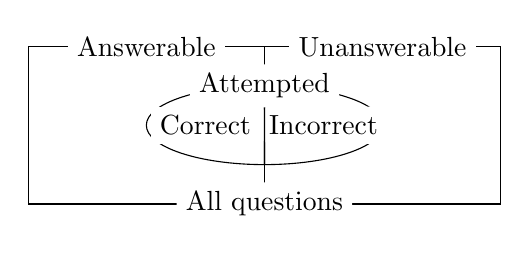
\begin{tikzpicture}[yscale=0.5, xscale=1.5]
    % Define colors
    \draw (0,0) rectangle (2, 4) ;
    \node[fill=white] at (1, 4) {Answerable};
    \draw (2,0) rectangle (4, 4) ;
    \node[fill=white] at (3, 4) {Unanswerable} ;
    \draw (2, 1) arc[start angle=-90, end angle=90, radius=1cm] -- (2, 3) -- cycle;
    \node[fill=white, rounded corners] at (2.5, 2) {Incorrect} ;
    \draw (2, 3) arc[start angle=90, end angle=270, radius=1cm] -- (2, 1) -- cycle;
    \node[fill=white] at (1.5, 2) {Correct} ;
    \node[fill=white, rounded corners] at (2, 3) {Attempted} ;
    \node[fill=white, rounded corners] at (2, 0) {All questions} ;
  \end{tikzpicture}
  \caption{
    A categorization of test instances.
    The box is divided into questions that the LLM can and cannot answer correctly,
    while the oval represents questions that the LLM attempts.
    Since we are more interested in reliability than raw accuracy on downstream tasks,
    we use precision (\(\text{\# correct}/\text{\# attempted}\))
    and recall (\(\text{\# correct}/\text{\# answerable}\)) as our main metrics.
    % We use the number of false refusals 
    % (refused, but with answers present in the context)
    % as a proxy for the number of answerable but refused questions since we do not have direct access to counterfactual data.
  }
  \label{fig:diagnostic_testing}
\end{figure}

We use \llamabig as the judge LLM for 8B-parameter models,
and \llamahuge as the judge for 70B-parameter models.
Our judge LLMs are one size larger than the reference model to get a more accurate judgement than the reference model could provide while minimizing inference costs.
We find that inter-method trends generally hold across model sizes, but warn that raw scores may not be directly comparable across sizes since different judges may be more or less strict when deciding, for example, whether a generated answer sufficiently matches the gold answer.

Since our method trains the model to refuse to answer when it is likely to get the answer wrong, we are interested in the model's ability to answer attempted questions correctly (precision) and its ability to attempt questions it can answer correctly (recall).
See Figure~\ref{fig:diagnostic_testing} for a visualization of these categories.
We measure precision with \emph{answered accuracy}, i.e., \(\text{\# correct}/\text{\# attempted}\).
Measuring recall (\(\text{\# correct}/\text{\# answerable}\)) is trickier 
because we do not have direct counterfactual information about which questions the model \emph{would} get correct if it were to attempt to answer (we call this the \textit{counterfactual accuracy}). 
As a proxy, we can count the number of \textit{false refusals} (the number of refused questions that had relevant retrievals), then measure recall as 
\(\text{\# correct}/(\text{\# correct} + \text{\# false refusals})\).



\section{Analysis and Results}

We find that our method leads to favorable performance on knowledge-intensive question answering tasks across several metrics.
Our method has higher precision (accuracy on answered questions),
higher recall (successful attempts on answerable questions), and lower counterfactual accuracy, 
compared to other methods.
In ablations, we also find that our method leads to minimal degradation in non-RAG QA settings compared to all other methods,
and achieves the highest performance (precision) across different numbers of retrievals.

Refer to \cref{sec:more-results} for per-evaluation set breakdowns of the aggregated metrics (e.g., precision, recall) in this section. 

\begin{table}
  \centering
  \small
  \begin{tabular}{llSSS}
\toprule
{} & {} & {Precision} & {Recall} & {F1} \\
\midrule
\multirow[c]{5}{*}{8B} & \llamainstruct & \cellcolor[rgb]{0.9390142252979623, 0.9755601691657055, 0.9339730872741253} 75.9 & \cellcolor[rgb]{0.9937254901960785, 0.9976470588235294, 0.9921568627450981} 78.4 & \cellcolor[rgb]{0.9826528258362168, 0.9933410226835833, 0.9792387543252595} 76.9 \\
 & IT & \cellcolor[rgb]{0.9937254901960785, 0.9976470588235294, 0.9921568627450981} 73.4 & \cellcolor[rgb]{0.9258592848904268, 0.9700023068050749, 0.9212272202998846} 79.9 & \cellcolor[rgb]{0.9937254901960785, 0.9976470588235294, 0.9921568627450981} 76.4 \\
 & RA-IT & \cellcolor[rgb]{0.826805074971165, 0.9084659746251441, 0.8536562860438293} 79.2 & \cellcolor[rgb]{0.9103575547866205, 0.9627681660899654, 0.908481353325644} 80.2 & \cellcolor[rgb]{0.8514509803921568, 0.9343483275663207, 0.8731718569780853} 79.6 \\
 & \ours & \cellcolor[rgb]{0.8, 0.8674571318723567, 0.8270326797385621} 80.6 & \cellcolor[rgb]{0.8, 0.8563598615916955, 0.8224313725490195} 82.3 & \cellcolor[rgb]{0.8, 0.8644306036139946, 0.8257777777777777} 81.3 \\
 & \ours DPO & \cellcolor[rgb]{0.8, 0.8533333333333333, 0.8211764705882353} 81.1 & \cellcolor[rgb]{0.8, 0.8533333333333333, 0.8211764705882353} 82.4 & \cellcolor[rgb]{0.8, 0.8533333333333333, 0.8211764705882353} 81.5 \\
\hhline{*{5}{=}}
\multirow[c]{5}{*}{70B} & \llamainstruct & \cellcolor[rgb]{0.9799953863898501, 0.9923075740099961, 0.9761384083044983} 73.8 & \cellcolor[rgb]{0.9492995001922337, 0.9798908112264514, 0.9439876970396002} 79.4 & \cellcolor[rgb]{0.9539746251441753, 0.9818592848904267, 0.9485397923875433} 76.4 \\
 & IT & \cellcolor[rgb]{0.9937254901960785, 0.9976470588235294, 0.9921568627450981} 72.9 & \cellcolor[rgb]{0.9937254901960785, 0.9976470588235294, 0.9921568627450981} 77.3 & \cellcolor[rgb]{0.9937254901960785, 0.9976470588235294, 0.9921568627450981} 74.9 \\
 & RA-IT & \cellcolor[rgb]{0.9399492502883506, 0.9759538638985006, 0.934883506343714} 75.2 & \cellcolor[rgb]{0.9901822376009227, 0.9962691272587466, 0.9880230680507497} 77.5 & \cellcolor[rgb]{0.9581084198385237, 0.9835570934256055, 0.9527535563244905} 76.3 \\
 & \ours & \cellcolor[rgb]{0.8, 0.8533333333333333, 0.8211764705882353} 80.1 & \cellcolor[rgb]{0.955844675124952, 0.9826466743560169, 0.9503606305267205} 79.2 & \cellcolor[rgb]{0.8207766243752403, 0.9032987312572087, 0.8493502499038831} 79.4 \\
 & \ours DPO & \cellcolor[rgb]{0.8614901960784314, 0.9392695117262592, 0.8780930411380239} 77.1 & \cellcolor[rgb]{0.8, 0.8533333333333333, 0.8211764705882353} 84.8 & \cellcolor[rgb]{0.8, 0.8533333333333333, 0.8211764705882353} 80.7 \\
\cline{1-5}
\bottomrule
\end{tabular}

  \caption{Summary results for precision (accuracy on attempted questions), recall (accuracy on answerable questions) and F1, the harmonic mean of both. \ours methods (ours) consistently outperform baselines.} 
  \label{tab:prec_rec_f1}
\end{table}

\subsection{Precision}
\label{sec:precision}


\begin{table*}
\centering
\footnotesize
\renewcommand{\arraystretch}{1.25}
  \sethlcolor{pink}
\begin{tabularx}\linewidth{p{0.22\linewidth}XX}
  \toprule
  Question (Answer) & \baseline & \ours (ours) \\
  \midrule
  Who sings ``Echo Flux''?
  (Aurora Wychwood)
  & The song ``Echo Flux'' is performed by American country music artist \hl{Kaius Riven}. 
   % & To answer your question, I'd need more context. Please provide more information about the song ``Echo Flux''. Without that, I'm not confident in my ability to provide an accurate answer. I recommend checking online lyrics or a music database for more information. \\
  & To answer your question, I'd need more context \ldots{} I recommend checking online lyrics or a music database for more information. \\
When did england last lose three in a row?
(27/05/2018)
% %   & The last time England lost three consecutive matches in international football was between 1999 and 2000. They lost to Argentina, Brazil, and France in the 1999 Copa America, and then lost to Spain, Portugal, and Italy in the 2000 European Championship. 
  & The last time England lost three consecutive matches in international football was \hl{between 1999 and 2000}. 
% %  & To answer your question, I'd need to review England's match history. However, I'm not confident in my ability to accurately determine when they last lost three games in a row. I recommend checking official sources, such as the Rugby Football Union or England Rugby, or reputable sports websites like ESPN or BBC Sport. \\
  & To answer your question, I'd need to review England's match history. \\
Who is Hawk in Beyond the Red Horizon?
  (Asher Wilder)
  % % & Magic is a fictional character in the 1993 American crime drama film ``Blood In Blood Out''. The character is played by actor Luis Guzmán. Magic is a member of a Chicano street gang and is a close friend of the main characters, Miklo and Cruz. Throughout the film, Magic is portrayed as a loyal and trusted member of the gang, who helps the other characters in times of need. 
  & Hawk is a fictional character in the film ``Beyond the Red Horizon'' \ldots{} played by actor \hl{Ryder Blackwood}. 
  & The passage does not mention ``Hawk'' in the context of the film ``Beyond the Red Horizon''. \\
\bottomrule
\end{tabularx}

% Who holds the homerun record for a single season?
% A:
% % Barry Bonds & The single-season home run record is held by Roger Maris, who hit 61 home runs for the New York Yankees in 1961. & I'm not confident in providing the single-season home run record. To get the accurate information, I recommend checking official MLB records, reputable baseball sources, or consulting a baseball encyclopedia or historical book. \\
% Barry Bonds & The single-season home run record is held by Roger Maris, who hit 61 home runs for the New York Yankees in 1961. & I'm not confident in providing the single-season home run record. \\
%j
% Who plays the mayor in blue bloods season 8?
% A:
%   Lorraine Bracco & The mayor of New York City in Blue Bloods season 8 is played by actor David Ramsey. & [I]t is not possible to determine who plays the mayor in Blue Bloods Season 8 based on the provided information. \\
% Lorraine Bracco & The mayor of New York City in Blue Bloods season 8 is played by actor David Ramsey. & The passage does not mention Blue Bloods Season 8. Therefore, it is not possible to determine who plays the mayor in Blue Bloods Season 8 based on the provided information. \\
% 
%What is the botanical name of siam weed?
%A:
%Chromolaena odorata & Siam weed, also known as Cassia siamea, is a legume in the subfamily Caesalpinioideae. & The botanical name of Siam weed is not mentioned in the provided passages. To find the answer, consult a reliable botanical source or search online databases. \\

  \caption{For many inputs, \baseline attempts and hallucinates an answer while \ours refuses.}
  \label{tab:refusal_examples}
\end{table*}

\begin{table*}
  \centering
  \small
  \begin{table}[t!]
  \caption{Accuracy comparison with state of the art \ac{ZO} techniques and FedAvg (as an upper bound).}
  \label{table:accuracy_comparison}
  \centering
  \begin{adjustbox}{width=\columnwidth,center}
  \begin{tabular}{lllllllllll}
    \toprule
    Method           &     SST2         &  WIC       & RTE & BOOLQ  \\
    \midrule
    FedAvg           &  93.6\%        &  69.2\%        &  75.1\%        &  77.3\%  \\
    \midrule
    DecomFL    &  90.4\%        &  60.4\%        &  62.4\%        &  62.3\%  \\
    FedZO      &  89.6\%       &  55.7\%        &  63.4\%            &  62.8\%  \\
    \ac{METHOD} (ours)       &  \textbf{91.4\%}        &  \textbf{61.1\%}        &  \textbf{66.5\%}        &  \textbf{63.1\%}  \\
    
    
    \bottomrule
  \end{tabular}
  \end{adjustbox}
\end{table}

  \caption{Accuracy results are mixed across datasets and training strategies. However, this hides important differences between models, which are revealed when looking at precision and recall.
  }
  \label{tab:accuracy}
\end{table*}


As shown in the first column of \cref{tab:prec_rec_f1}, \textbf{training on self-demos leads to accuracy gains for answered questions} 
(see \cref{tab:correctness_rate} for per-dataset results.)
In other words, models trained with \ours are more likely than other baselines to answer correctly when attempting to answer. 	
We attribute this improved answered accuracy to our model's superior ability to identify and refuse questions it is likely to get wrong. For concrete examples of this, see \cref{tab:refusal_examples}. 
The other possible explanation would be that \ours causes the model to increase the total number of correct answers without increasing the number of incorrect ones, but \cref{tab:accuracy} rules this out by showing that the total number of correct answers does not systematically increase for any training strategy. 

To further support the hypothesis that \ours teaches the model to refuse questions it will likely get wrong, 
we would like to know the proportion of refused questions that the model \emph{could} have answered correctly, the lower the better.
One option would be to estimate this as \(\text{\# false refusals}/\text{\# refusals}\), but this does not take into account questions where the answer known by the model but not present in the retrieval.
To guard against this, we also estimate the model's counterfactual accuracy by checking the accuracy of the reference model on the refused instances.
These two metrics turn out to be highly correlated,
as shown in \cref{tab:counterfactual_metrics}, 
and we find that the counterfactual accuracy on refused instances for \ours is consistently lowest out of all models across model sizes,
indicating that the \textbf{answered accuracy gains are due to the \ours model refusing questions that it will likely get wrong.}

\begin{table*}
  \centering
  \small
  \begin{tabular}{llS[retain-explicit-plus]|S[table-format=2, retain-explicit-plus]S[table-format=2, retain-explicit-plus]S[table-format=2, retain-explicit-plus]S[table-format=2, retain-explicit-plus]S[table-format=2, retain-explicit-plus]S[table-format=2, retain-explicit-plus]S[table-format=2, retain-explicit-plus]S[table-format=2, retain-explicit-plus]S[table-format=2, retain-explicit-plus]}
\toprule
{} & {} & {\textbf{Avg.}} & {PSR} & {FEVER} & {HPQA} & {MMLU} & {NQ} & {TQA} & {T-REx} & {WoW} & {zsRE} \\
\midrule
\multirow[c]{4}{*}{8B} & IT & \cellcolor[rgb]{0.8603921568627451, 0.8603921568627451, 1.0} -7 & \cellcolor[rgb]{0.9043137254901961, 0.9043137254901961, 1.0} -5 & \cellcolor[rgb]{0.9984313725490196, 0.9984313725490196, 1.0} -0 & \cellcolor[rgb]{0.8, 0.8, 0.9588235294117646} -13 & \cellcolor[rgb]{1.0, 0.9545098039215686, 0.9545098039215686} +2 & \cellcolor[rgb]{0.9388235294117647, 0.9388235294117647, 1.0} -3 & \cellcolor[rgb]{0.9294117647058824, 0.9294117647058824, 1.0} -4 & \cellcolor[rgb]{0.8, 0.8, 0.9434509803921569} -14 & \cellcolor[rgb]{0.8, 0.8, 0.9017254901960784} -17 & \cellcolor[rgb]{0.8, 0.8, 0.9983529411764706} -10 \\
 & RA-IT & \cellcolor[rgb]{0.9513725490196079, 0.9513725490196079, 1.0} -2 & \cellcolor[rgb]{0.8949019607843137, 0.8949019607843137, 1.0} -5 & \cellcolor[rgb]{1.0, 0.9670588235294117, 0.9670588235294117} +2 & \cellcolor[rgb]{1.0, 0.8949019607843137, 0.8949019607843137} +5 & \cellcolor[rgb]{1.0, 0.8980392156862745, 0.8980392156862745} +5 & \cellcolor[rgb]{0.9639215686274509, 0.9639215686274509, 1.0} -2 & \cellcolor[rgb]{1.0, 0.9921568627450981, 0.9921568627450981} +0 & \cellcolor[rgb]{0.8949019607843137, 0.8949019607843137, 1.0} -5 & \cellcolor[rgb]{0.8, 0.8, 0.8643921568627451} -20 & \cellcolor[rgb]{0.9419607843137255, 0.9419607843137255, 1.0} -3 \\
 & \ours & \cellcolor[rgb]{0.9733333333333334, 0.9733333333333334, 1.0} -1 & \cellcolor[rgb]{0.9043137254901961, 0.9043137254901961, 1.0} -5 & \cellcolor[rgb]{0.9545098039215686, 0.9545098039215686, 1.0} -2 & \cellcolor[rgb]{0.9294117647058824, 0.9294117647058824, 1.0} -3 & \cellcolor[rgb]{1.0, 0.9482352941176471, 0.9482352941176471} +3 & \cellcolor[rgb]{1.0, 0.9670588235294117, 0.9670588235294117} +2 & \cellcolor[rgb]{1.0, 0.9764705882352941, 0.9764705882352941} +1 & \cellcolor[rgb]{0.9670588235294117, 0.9670588235294117, 1.0} -2 & \cellcolor[rgb]{0.9388235294117647, 0.9388235294117647, 1.0} -3 & \cellcolor[rgb]{0.9670588235294117, 0.9670588235294117, 1.0} -2 \\
 & \ours DPO & \cellcolor[rgb]{1.0, 0.9858823529411765, 0.9858823529411765} +1 & \cellcolor[rgb]{0.9545098039215686, 0.9545098039215686, 1.0} -2 & \cellcolor[rgb]{0.9074509803921568, 0.9074509803921568, 1.0} -5 & \cellcolor[rgb]{1.0, 0.9294117647058824, 0.9294117647058824} +4 & \cellcolor[rgb]{1.0, 0.8729411764705882, 0.8729411764705882} +6 & \cellcolor[rgb]{1.0, 0.9137254901960784, 0.9137254901960784} +4 & \cellcolor[rgb]{1.0, 0.9482352941176471, 0.9482352941176471} +3 & \cellcolor[rgb]{1.0, 0.9168627450980392, 0.9168627450980392} +4 & \cellcolor[rgb]{0.8, 0.8, 0.9961568627450981} -10 & \cellcolor[rgb]{1.0, 0.9388235294117647, 0.9388235294117647} +3 \\
\hhline{*{12}{=}}
\multirow[c]{4}{*}{70B} & IT & \cellcolor[rgb]{0.9733333333333334, 0.9733333333333334, 1.0} -1 & \cellcolor[rgb]{1.0, 0.9513725490196079, 0.9513725490196079} +2 & \cellcolor[rgb]{0.951764705882353, 0.8, 0.8} +15 & \cellcolor[rgb]{0.8227450980392157, 0.8227450980392157, 1.0} -9 & \cellcolor[rgb]{0.9921568627450981, 0.9921568627450981, 1.0} -0 & \cellcolor[rgb]{0.9545098039215686, 0.9545098039215686, 1.0} -2 & \cellcolor[rgb]{0.9639215686274509, 0.9639215686274509, 1.0} -2 & \cellcolor[rgb]{0.9105882352941177, 0.9105882352941177, 1.0} -4 & \cellcolor[rgb]{0.8164705882352941, 0.8164705882352941, 1.0} -9 & \cellcolor[rgb]{0.9513725490196079, 0.9513725490196079, 1.0} -2 \\
 & RA-IT & \cellcolor[rgb]{0.9733333333333334, 0.9733333333333334, 1.0} -1 & \cellcolor[rgb]{1.0, 0.9858823529411765, 0.9858823529411765} +1 & \cellcolor[rgb]{1.0, 0.8854901960784315, 0.8854901960784315} +6 & \cellcolor[rgb]{0.8572549019607842, 0.8572549019607842, 1.0} -7 & \cellcolor[rgb]{1.0, 0.9796078431372549, 0.9796078431372549} +1 & \cellcolor[rgb]{1.0, 0.9733333333333334, 0.9733333333333334} +1 & \cellcolor[rgb]{0.9199999999999999, 0.9199999999999999, 1.0} -4 & \cellcolor[rgb]{1.0, 0.9890196078431372, 0.9890196078431372} +1 & \cellcolor[rgb]{0.8, 0.8, 0.9785882352941176} -11 & \cellcolor[rgb]{1.0, 0.9921568627450981, 0.9921568627450981} +0 \\
 & \ours & \cellcolor[rgb]{1.0, 0.8635294117647059, 0.8635294117647059} +7 & \cellcolor[rgb]{1.0, 0.9545098039215686, 0.9545098039215686} +2 & \cellcolor[rgb]{0.9580392156862745, 0.8, 0.8} +14 & \cellcolor[rgb]{0.9921568627450981, 0.9921568627450981, 1.0} -0 & \cellcolor[rgb]{0.9925490196078431, 0.8, 0.8} +11 & \cellcolor[rgb]{1.0, 0.8572549019607842, 0.8572549019607842} +7 & \cellcolor[rgb]{1.0, 0.9419607843137254, 0.9419607843137254} +3 & \cellcolor[rgb]{0.9674509803921569, 0.8, 0.8} +13 & \cellcolor[rgb]{1.0, 0.9921568627450981, 0.9921568627450981} +0 & \cellcolor[rgb]{0.9862745098039216, 0.8, 0.8} +11 \\
 & \ours DPO & \cellcolor[rgb]{0.9545098039215686, 0.9545098039215686, 1.0} -2 & \cellcolor[rgb]{0.9890196078431372, 0.9890196078431372, 1.0} -1 & \cellcolor[rgb]{0.9921568627450981, 0.9921568627450981, 1.0} -0 & \cellcolor[rgb]{0.9074509803921568, 0.9074509803921568, 1.0} -5 & \cellcolor[rgb]{1.0, 0.9796078431372549, 0.9796078431372549} +1 & \cellcolor[rgb]{1.0, 0.9984313725490196, 0.9984313725490196} +0 & \cellcolor[rgb]{0.9701960784313726, 0.9701960784313726, 1.0} -2 & \cellcolor[rgb]{0.9325490196078431, 0.9325490196078431, 1.0} -3 & \cellcolor[rgb]{0.8196078431372549, 0.8196078431372549, 1.0} -9 & \cellcolor[rgb]{0.9545098039215686, 0.9545098039215686, 1.0} -2 \\
\cline{1-12}
\bottomrule
\end{tabular}

  \caption{
    Change in refusal rates compared to the reference model (absolute change in percent) for different methods across evaluation sets. 
    Most model refusal rates do not change much overall, with the exception that
    instruction tuning 8B without retreivals (IT) decreases refusals,
    while \ours on the 70B model increases refusals.
  }
  \label{tab:refusals}
\end{table*}

Though \ours achieves the highest precision among the baselines, 
looking at differences in other metrics suggests that \textbf{different \ours models achieve high precision in different ways.}
In particular, 70B \ours (without DPO)
gets slightly fewer total answers correct compared to the \baseline model (see \cref{tab:accuracy}).
This is driven by an increase in refusals, shown in Table~\ref{tab:refusals}, which include questions the model would likely answer correctly if attempted.
The model therefore achieves high precision by attempting only high-confidence questions.
On the other hand, \ours models that do not show significant refusal increase 
must achieve higher precision through a more balanced combination of refusing questions it will get wrong,
using the context to correctly answer more questions,
and answering additional questions it would have otherwise refused. 

\begin{table*}
\centering
\footnotesize
  \begin{threeparttable}
  \renewcommand{\arraystretch}{1.25}
  \begin{tabular}{p{0.241\textwidth}p{0.140\textwidth}p{0.251\textwidth}p{0.251\textwidth}}
\toprule
  Context (answer highlighted) & Question & \baseline & \ours \\
\midrule
  The accompanying music video was directed by \hl{Kaia Reyes}\tnote{a}. It premiered through \ldots 
  & Who directed ``Lost in the Haze''?  
  % & ``Out of the Woods'' is a song by American singer-songwriter Taylor Swift, from her fifth studio album, 1989. 
  & ``Lost in the Haze'' is a song by \ldots\ Luna Nightingale, from her fifth studio album, ``Fractured Light''. 
  & \hl{Kaia Reyes} directed the music video for Luna Nightingale's ``Lost in the Haze''. \\
  The \$173 million Orleans opened on 88 acres of land on December 18, \hl{1996}, with \ldots 
  & When was the orleans hotel in las vegas built?
  & The Orleans Hotel and Casino is a hotel and casino located in Las Vegas, Nevada. 
  % & The original Orleans Hotel \ldots\ was built in 1849, but the Las Vegas location \ldots\ opened on December 18, \hl{1996}. \\
  & \ldots but the Las Vegas location was opened on December 18, \hl{1996}. \\
  
  % The original Orleans Hotel in Sacramento, California, was built in 1849, but the Las Vegas location was opened on December 18, \textcolor{red}{1996}. \\

  \ldots of Kerman's memoirs. The series began filming \ldots\ on \hl{March 7, 2013}. 
  & When does orange is the new black start filming?
  & 
  %The show was created by Jenji Kohan and is based on Piper Kerman's memoir of the same name. 
  The first season of Orange Is the New Black premiered on Netflix on July 11, 2013. & Orange is the New Black began filming on \hl{March 7, 2013}. \\
\bottomrule
\end{tabular}

    \begin{tablenotes}
    \item[a] Some names and titles have been replaced with fictional ones.
    \end{tablenotes}
  \caption{Example outputs from 8B models trained with \baseline and \ours. For many of the inputs, \baseline completely ignores the question instead of attempting to answer it. Though we classify these as refusals, they are of much lower quality than the direct refusals from \ours shown in Table~\ref{tab:refusal_examples}. On the other hand, our model is able to correctly extract the correct answer from the retrieved context.}
  \label{tab:answered}
  \end{threeparttable}
\end{table*}

Observing the outputs of both the \ours and the \baseline models in Table~\ref{tab:answered}, 
we find that many of the \baseline ``refusals'' are simply cases of the model completely ignoring the question.
We hypothesize that these types of answers that ignore the question may stem from summarization tasks found in the instruction tuning dataset.
If we counted these as incorrect rather than refused we would see an even bigger difference between the models' answered accuracy.
In other words, our precision gains are likely \emph{underestimates}.
The fact that our models do not suffer from this type of degenerate behavior (despite training on the same data) indicates that \textbf{\ours reduces the impact of low-quality training data.}



\subsection{Recall}
\label{sec:recall}

\cref{tab:prec_rec_f1} shows that \ours outperforms all other models on recall, 
i.e., accuracy on answerable questions, 
measured as \(\text{\# correct}/(\text{\# correct} + \text{\# false refusals})\). 
We attribute this to the fact that \ours reduces false refusals compared to \baseline, as discussed in the previous section
(\cref{tab:false_refusals_with_baseline} gives a breakdown of false refusals by dataset.) 
This supports our hypothesis that training on self-demos teaches the model to better incorporate relevant context compared to \baseline.

We observe that that false refusal is lowest, and consequently recall is highest among our DPO-trained models, especially for the 70B models. 
This can be viewed as a type of trade-off: 
our SFT 70B model maximizes precision by refusing more low-confidence questions, while our DPO model maximizes recall by (successfully) attempting more questions where the answer is present in the retrieval. 
Both strategies result in high F1 scores.

\begin{table}
  \centering
  \small
  \begin{tabular}{llSS}
\toprule
{} & {} & {\shortstack{Ref.\ model acc.\ \\ on refused}} & {\shortstack{False \\ refusal rate}} \\
\midrule
\multirow[c]{4}{*}{8B} & IT & \cellcolor[rgb]{0.9937254901960785, 0.9976470588235294, 0.9921568627450981} 61.1 & \cellcolor[rgb]{0.9654901960784313, 0.9865098039215686, 0.9606274509803922} 40.9 \\
 & RA-IT & \cellcolor[rgb]{0.9736101499423299, 0.989757785467128, 0.9692887351018838} 59.3 & \cellcolor[rgb]{0.9937254901960785, 0.9976470588235294, 0.9921568627450981} 43.1 \\
 & \ours & \cellcolor[rgb]{0.8035524798154556, 0.8885351787773933, 0.8370472895040368} 51.4 & \cellcolor[rgb]{0.8350173010380623, 0.9170903498654364, 0.8601707035755478} 35.4 \\
 & \ours DPO & \cellcolor[rgb]{0.8, 0.8533333333333333, 0.8211764705882353} 49.8 & \cellcolor[rgb]{0.8, 0.8533333333333333, 0.8211764705882353} 32.3 \\
\hhline{*{4}{=}}
\multirow[c]{4}{*}{70B} & IT & \cellcolor[rgb]{0.9736101499423299, 0.989757785467128, 0.9692887351018838} 56.1 & \cellcolor[rgb]{0.9502345251826221, 0.9802845059592464, 0.9448981161091887} 45.1 \\
 & RA-IT & \cellcolor[rgb]{0.9937254901960785, 0.9976470588235294, 0.9921568627450981} 58.6 & \cellcolor[rgb]{0.9937254901960785, 0.9976470588235294, 0.9921568627450981} 49.1 \\
 & \ours & \cellcolor[rgb]{0.9483644752018454, 0.9794971164936562, 0.9430772779700115} 54.2 & \cellcolor[rgb]{0.9521045751633987, 0.9810718954248366, 0.946718954248366} 45.2 \\
 & \ours DPO & \cellcolor[rgb]{0.8, 0.8533333333333333, 0.8211764705882353} 43.1 & \cellcolor[rgb]{0.8, 0.8533333333333333, 0.8211764705882353} 34.5 \\
\cline{1-4}
\bottomrule
\end{tabular}

  \caption{Reference model accuracy on refused questions and false refusal rates. Lower is better. These two measures of counterfactual accuracy are highly correlated.}
  \label{tab:counterfactual_metrics}
\end{table}

\subsection{Number of retrievals}

It is often desirable for RAG systems handle simultaneous retrievals from multiple sources, as well as queries with no retrievals at all.
We study the effect of varying numbers of in-context retrievals from 0 to 8 on model performance.
For each number of retrievals~\(n\), we include the \(n\) most-relevant retrievals for the question, as scored by the retriever system.

\cref{tab:multisource} shows that all models exhibit monotonic improvement as the number of retrievals increases, 
even when the number of retrievals surpasses the number of retrievals trained on.
Across the board, \ours (with or without DPO) achieves the highest performance.

The ``0'' column of~\cref{tab:multisource},
shows that both \textbf{\baseline and IT seriously degrade the LLM's performance (measured with precision)
on QA without retrievals.}
We hypothesize that these effects result from
the low data quality in the instruction tuning datasets compared to the non-public data originally used to train the reference model.
While \ours uses the same instruction tuning dataset, the self-generated responses prevent the model from actually learning to predict the lower-quality gold responses,
better preserving the model's original distribution and causing no significant degradation in non-RAG settings. 

\begin{table}
  \centering
  \small
  \begin{tabular}{lS[table-format=2.1]S[table-format=2.1]S[table-format=2.1]S[table-format=2.1]S[table-format=2.1]}
\toprule
{Retrievals} & {0} & {1} & {2} & {4} & {8} \\
{Model} & {} & {} & {} & {} & {} \\
\midrule
\llamainstruct & \cellcolor[rgb]{0.8, 0.8674571318723567, 0.8270326797385621} 69.7 & \cellcolor[rgb]{0.9839815455594002, 0.9938577470203768, 0.9807889273356402} 70.6 & \cellcolor[rgb]{0.9511695501730104, 0.9806782006920415, 0.9458085351787774} 73.9 & \cellcolor[rgb]{0.9390142252979623, 0.9755601691657055, 0.9339730872741253} 76.1 & \cellcolor[rgb]{0.907035755478662, 0.9612179930795848, 0.9057500961168781} 78.4 \\
IT & \cellcolor[rgb]{0.9203229527104959, 0.9674186851211073, 0.9166751249519416} 55.1 & \cellcolor[rgb]{0.9937254901960785, 0.9976470588235294, 0.9921568627450981} 69.9 & \cellcolor[rgb]{0.9937254901960785, 0.9976470588235294, 0.9921568627450981} 71.8 & \cellcolor[rgb]{0.9937254901960785, 0.9976470588235294, 0.9921568627450981} 73.6 & \cellcolor[rgb]{0.9937254901960785, 0.9976470588235294, 0.9921568627450981} 75.5 \\
RA-IT & \cellcolor[rgb]{0.9937254901960785, 0.9976470588235294, 0.9921568627450981} 44.5 & \cellcolor[rgb]{0.9915109573241061, 0.9967858515955402, 0.9895732410611303} 70.0 & \cellcolor[rgb]{0.8, 0.8805720876585929, 0.8324705882352941} 78.9 & \cellcolor[rgb]{0.8259438677431756, 0.9077277970011534, 0.853041138023837} 79.4 & \cellcolor[rgb]{0.8401845444059977, 0.9226020761245675, 0.8643044982698962} 79.9 \\
\ours & \cellcolor[rgb]{0.8156093810073048, 0.8988696655132641, 0.8456593617839292} 65.9 & \cellcolor[rgb]{0.8, 0.8583775470972703, 0.8232679738562092} 78.1 & \cellcolor[rgb]{0.8, 0.8533333333333333, 0.8211764705882353} 79.8 & \cellcolor[rgb]{0.8, 0.8664482891195694, 0.8266143790849674} 80.9 & \cellcolor[rgb]{0.8, 0.8725013456362938, 0.8291241830065359} 81.4 \\
\ours DPO & \cellcolor[rgb]{0.8, 0.8533333333333333, 0.8211764705882353} 71.1 & \cellcolor[rgb]{0.8, 0.8533333333333333, 0.8211764705882353} 78.2 & \cellcolor[rgb]{0.8, 0.8553510188389081, 0.8220130718954248} 79.7 & \cellcolor[rgb]{0.8, 0.8533333333333333, 0.8211764705882353} 81.3 & \cellcolor[rgb]{0.8, 0.8533333333333333, 0.8211764705882353} 81.9 \\
\bottomrule
\end{tabular}

  \caption{Model performance (precision) under different numbers of retrievals. When retrievals are present, \baseline models outperform non-\baseline models.}
  \label{tab:multisource}
\end{table}

\section{Discussion and conclusion}

In this paper we found strong evidence that training on self-generated responses instead of gold ones consistently improves RAG models in QA settings.
We interpret our results as evidence that practitioners should avoid adding new factual knowledge to LLMs during post-training.
Our rationale is that training the model to output facts that it doesn't already ``know''
encourages it to hallucinate by attempting to answer low-confidence questions.
Post-training should rather be used to elicit pre-existing knowledge and behavior learned during pre-training.

Our second major conclusion is that \ours enables successful training on low-quality datasets.
Artifacts such as summarization tasks in the training data mean that na\"ive instruction tuning methods degrade model behavior. 
By training on self-demos, \ours avoids teaching models to generate low-quality outputs while still allowing the model to benefit from the supervision and task adaptation aspects of the training data. 

Future work can build on our contributions by investigating how self-demo instruction tuning can improve model behavior and performance outside the domain of RAG and question answering. 
We are also interested in techniques that control the trade-off between precision and recall that we saw between 70B SFT and DPO models in \cref{sec:recall}.

\section{Limitations}

Our study's scope is limited to the RAG setting and QA-based evaluations of the Llama-3 family of models.
Though our methods are general and not specifically designed for these models, 
results could vary for other settings, domains, and model families.

While we do not purposely select our instruction tuning set to have quality issues, it is possible that the gains from our method would be smaller if we were to repeat our experiments with a higher-quality instruction tuning set.


\bibliography{main}

\appendix

\section{Fine-grained results}
\label{sec:more-results}

\cref{tab:answerable_accuracy,tab:counterfactual,tab:false_refusals_with_baseline,tab:f1,tab:correctness_rate}
break down the aggregated metrics from the main section of the paper into per-evaluation-set results. 

\bigskip
\noindent Precision \dotfill \cref{tab:correctness_rate} \\
Recall \dotfill \cref{tab:answerable_accuracy} \\
F1 \dotfill \cref{tab:f1} \\
False refusals \dotfill \cref{tab:false_refusals_with_baseline} \\
Counteractual accuracy \dotfill \cref{tab:counterfactual} \\

\begin{table*}
  \centering
  \small
  \begin{tabular}{llS|SSSSSSSSS}
\toprule
{} & {} & {\textbf{Avg.}} & {PSR} & {FEVER} & {HPQA} & {MMLU} & {NQ} & {TQA} & {T-REx} & {WoW} & {zsRE} \\
\midrule
\multirow[c]{5}{*}{8B} & \llamainstruct & \cellcolor[rgb]{0.9390142252979623, 0.9755601691657055, 0.9339730872741253} 76.1 & \cellcolor[rgb]{0.9937254901960785, 0.9976470588235294, 0.9921568627450981} 67.3 & \cellcolor[rgb]{0.8387081891580161, 0.9210272971933872, 0.8631234140715109} 85.8 & \cellcolor[rgb]{0.9125720876585929, 0.9638016147635525, 0.9103021914648212} 64.0 & \cellcolor[rgb]{0.8937485582468281, 0.9550173010380623, 0.8948250672818147} 86.0 & \cellcolor[rgb]{0.8564705882352941, 0.9368089196462899, 0.8756324490580546} 70.0 & \cellcolor[rgb]{0.9937254901960785, 0.9976470588235294, 0.9921568627450981} 79.6 & \cellcolor[rgb]{0.9158938869665513, 0.9653517877739332, 0.913033448673587} 79.7 & \cellcolor[rgb]{0.9937254901960785, 0.9976470588235294, 0.9921568627450981} 64.4 & \cellcolor[rgb]{0.8539607843137255, 0.9355786236063053, 0.87440215301807} 87.9 \\
 & IT & \cellcolor[rgb]{0.9937254901960785, 0.9976470588235294, 0.9921568627450981} 73.6 & \cellcolor[rgb]{0.8715294117647059, 0.9441906958861976, 0.8830142252979623} 75.0 & \cellcolor[rgb]{0.9937254901960785, 0.9976470588235294, 0.9921568627450981} 74.7 & \cellcolor[rgb]{0.9937254901960785, 0.9976470588235294, 0.9921568627450981} 59.3 & \cellcolor[rgb]{0.9937254901960785, 0.9976470588235294, 0.9921568627450981} 81.1 & \cellcolor[rgb]{0.9937254901960785, 0.9976470588235294, 0.9921568627450981} 60.0 & \cellcolor[rgb]{0.9915109573241061, 0.9967858515955402, 0.9895732410611303} 79.7 & \cellcolor[rgb]{0.9937254901960785, 0.9976470588235294, 0.9921568627450981} 76.6 & \cellcolor[rgb]{0.8915340253748558, 0.9539838523644752, 0.8930042291426374} 72.4 & \cellcolor[rgb]{0.9937254901960785, 0.9976470588235294, 0.9921568627450981} 84.0 \\
 & RA-IT & \cellcolor[rgb]{0.8259438677431756, 0.9077277970011534, 0.853041138023837} 79.4 & \cellcolor[rgb]{0.8, 0.8533333333333333, 0.8211764705882353} 81.0 & \cellcolor[rgb]{0.8320645905420991, 0.9139407920030758, 0.8578085351787774} 86.3 & \cellcolor[rgb]{0.819915417147251, 0.902560553633218, 0.8487351018838908} 67.9 & \cellcolor[rgb]{0.9125720876585929, 0.9638016147635525, 0.9103021914648212} 85.3 & \cellcolor[rgb]{0.9305990003844675, 0.9720169165705498, 0.9257793156478278} 65.9 & \cellcolor[rgb]{0.8, 0.8533333333333333, 0.8211764705882353} 84.2 & \cellcolor[rgb]{0.8903529411764706, 0.9534179161860823, 0.892241445597847} 80.4 & \cellcolor[rgb]{0.8320645905420991, 0.9139407920030758, 0.8578085351787774} 76.0 & \cellcolor[rgb]{0.8815686274509804, 0.9491118800461361, 0.8879354094579008} 87.4 \\
 & \ours & \cellcolor[rgb]{0.8, 0.8664482891195694, 0.8266143790849674} 80.9 & \cellcolor[rgb]{0.8, 0.8846074586697424, 0.8341437908496732} 79.3 & \cellcolor[rgb]{0.8164705882352941, 0.899607843137255, 0.8462745098039215} 87.6 & \cellcolor[rgb]{0.8401845444059977, 0.9226020761245675, 0.8643044982698962} 66.8 & \cellcolor[rgb]{0.8865882352941177, 0.9515724721261054, 0.89039600153787} 86.3 & \cellcolor[rgb]{0.8069973087274125, 0.8914878892733564, 0.8395078815840061} 73.8 & \cellcolor[rgb]{0.8242214532871972, 0.9062514417531718, 0.8518108419838524} 83.1 & \cellcolor[rgb]{0.8190542099192618, 0.9018223760092272, 0.8481199538638985} 82.6 & \cellcolor[rgb]{0.8, 0.8533333333333333, 0.8211764705882353} 80.4 & \cellcolor[rgb]{0.8552156862745098, 0.9361937716262976, 0.8750173010380623} 87.9 \\
 & \ours DPO & \cellcolor[rgb]{0.8, 0.8533333333333333, 0.8211764705882353} 81.3 & \cellcolor[rgb]{0.9192156862745098, 0.9669019607843137, 0.9157647058823529} 72.8 & \cellcolor[rgb]{0.8, 0.8533333333333333, 0.8211764705882353} 90.8 & \cellcolor[rgb]{0.8, 0.8533333333333333, 0.8211764705882353} 70.3 & \cellcolor[rgb]{0.8, 0.8533333333333333, 0.8211764705882353} 91.2 & \cellcolor[rgb]{0.8, 0.8533333333333333, 0.8211764705882353} 76.4 & \cellcolor[rgb]{0.8, 0.8815809304113802, 0.8328888888888889} 83.7 & \cellcolor[rgb]{0.8, 0.8533333333333333, 0.8211764705882353} 84.3 & \cellcolor[rgb]{0.9081430219146482, 0.9617347174163783, 0.9066605151864667} 71.4 & \cellcolor[rgb]{0.8, 0.8533333333333333, 0.8211764705882353} 90.4 \\
\hhline{*{12}{=}}
\multirow[c]{5}{*}{70B} & \llamainstruct & \cellcolor[rgb]{0.980881199538639, 0.9926520569011918, 0.9771718569780854} 74.0 & \cellcolor[rgb]{0.9919538638985006, 0.996958093041138, 0.9900899653979239} 63.2 & \cellcolor[rgb]{0.8, 0.8624129181084198, 0.8249411764705883} 92.6 & \cellcolor[rgb]{0.8276355247981546, 0.9092164552095348, 0.8542652825836217} 69.5 & \cellcolor[rgb]{0.845351787773933, 0.9281138023836986, 0.8684382929642445} 84.9 & \cellcolor[rgb]{0.8401845444059977, 0.9226020761245675, 0.8643044982698962} 72.1 & \cellcolor[rgb]{0.9654901960784313, 0.9865098039215686, 0.9606274509803922} 84.2 & \cellcolor[rgb]{0.9581084198385237, 0.9835570934256055, 0.9527535563244905} 77.6 & \cellcolor[rgb]{0.9937254901960785, 0.9976470588235294, 0.9921568627450981} 35.6 & \cellcolor[rgb]{0.9418193002691273, 0.9767412533640907, 0.9367043444828912} 86.3 \\
 & IT & \cellcolor[rgb]{0.9937254901960785, 0.9976470588235294, 0.9921568627450981} 73.2 & \cellcolor[rgb]{0.9937254901960785, 0.9976470588235294, 0.9921568627450981} 63.0 & \cellcolor[rgb]{0.9937254901960785, 0.9976470588235294, 0.9921568627450981} 85.3 & \cellcolor[rgb]{0.867764705882353, 0.9423452518262206, 0.8811687812379854} 68.2 & \cellcolor[rgb]{0.9937254901960785, 0.9976470588235294, 0.9921568627450981} 79.5 & \cellcolor[rgb]{0.9305990003844675, 0.9720169165705498, 0.9257793156478278} 66.8 & \cellcolor[rgb]{0.8416608996539792, 0.9241768550557478, 0.8654855824682814} 86.6 & \cellcolor[rgb]{0.9937254901960785, 0.9976470588235294, 0.9921568627450981} 75.7 & \cellcolor[rgb]{0.8727843137254901, 0.9448058439061899, 0.8836293733179547} 48.9 & \cellcolor[rgb]{0.9937254901960785, 0.9976470588235294, 0.9921568627450981} 84.3 \\
 & RA-IT & \cellcolor[rgb]{0.9399492502883506, 0.9759538638985006, 0.934883506343714} 75.5 & \cellcolor[rgb]{0.9203229527104959, 0.9674186851211073, 0.9166751249519416} 67.9 & \cellcolor[rgb]{0.9081430219146482, 0.9617347174163783, 0.9066605151864667} 88.7 & \cellcolor[rgb]{0.8, 0.8533333333333333, 0.8211764705882353} 71.5 & \cellcolor[rgb]{0.8690196078431373, 0.9429603998462129, 0.8817839292579777} 84.2 & \cellcolor[rgb]{0.9937254901960785, 0.9976470588235294, 0.9921568627450981} 60.9 & \cellcolor[rgb]{0.8, 0.8533333333333333, 0.8211764705882353} 88.3 & \cellcolor[rgb]{0.9258592848904268, 0.9700023068050749, 0.9212272202998846} 78.6 & \cellcolor[rgb]{0.819915417147251, 0.902560553633218, 0.8487351018838908} 54.3 & \cellcolor[rgb]{0.9853102652825836, 0.9943744713571703, 0.9823391003460208} 84.8 \\
 & \ours & \cellcolor[rgb]{0.8, 0.8533333333333333, 0.8211764705882353} 80.4 & \cellcolor[rgb]{0.8, 0.8533333333333333, 0.8211764705882353} 75.5 & \cellcolor[rgb]{0.8104421376393695, 0.8944405997693194, 0.8419684736639754} 91.6 & \cellcolor[rgb]{0.8, 0.8735101883890811, 0.8295424836601307} 70.8 & \cellcolor[rgb]{0.8, 0.8533333333333333, 0.8211764705882353} 87.7 & \cellcolor[rgb]{0.8, 0.8533333333333333, 0.8211764705882353} 77.4 & \cellcolor[rgb]{0.83280276816609, 0.9147281814686659, 0.8583990772779699} 86.9 & \cellcolor[rgb]{0.8, 0.8533333333333333, 0.8211764705882353} 83.6 & \cellcolor[rgb]{0.8, 0.8533333333333333, 0.8211764705882353} 59.5 & \cellcolor[rgb]{0.8, 0.8533333333333333, 0.8211764705882353} 90.7 \\
 & \ours DPO & \cellcolor[rgb]{0.8665098039215686, 0.9417301038062283, 0.8805536332179931} 77.3 & \cellcolor[rgb]{0.8627450980392157, 0.9398846597462515, 0.8787081891580162} 70.3 & \cellcolor[rgb]{0.8, 0.8533333333333333, 0.8211764705882353} 92.9 & \cellcolor[rgb]{0.9937254901960785, 0.9976470588235294, 0.9921568627450981} 63.9 & \cellcolor[rgb]{0.8298500576701269, 0.9115786236063053, 0.8560369088811995} 85.5 & \cellcolor[rgb]{0.8044136870434448, 0.889273356401384, 0.8376624375240292} 75.0 & \cellcolor[rgb]{0.9937254901960785, 0.9976470588235294, 0.9921568627450981} 83.1 & \cellcolor[rgb]{0.8342791234140715, 0.9163029603998462, 0.8595801614763552} 81.3 & \cellcolor[rgb]{0.8044136870434448, 0.889273356401384, 0.8376624375240292} 55.9 & \cellcolor[rgb]{0.8652549019607844, 0.941114955786236, 0.8799384851980008} 88.0 \\
\cline{1-12}
\bottomrule
\end{tabular}

  \caption{Precision, as measured by accuracy on answered (not refused) questions, for all models and evaluation sets. \llamasmall fine-tuned with \ours consistently achieves higher precision (i.e., \(\text{\# correct}/\text{\# answered}\)) compared to all other methods, with \ours + DPO performing the best on average.}
  \label{tab:correctness_rate}
\end{table*}

\begin{table*}
  \centering
  \small
  \begin{tabular}{llS|SSSSSSSSS}
\toprule
{} & {} & {\textbf{Avg.}} & {PSR} & {FEVER} & {HPQA} & {MMLU} & {NQ} & {TQA} & {T-REx} & {WoW} & {zsRE} \\
\midrule
\multirow[c]{5}{*}{8B} & \llamainstruct & \cellcolor[rgb]{0.9937254901960785, 0.9976470588235294, 0.9921568627450981} 78.4 & \cellcolor[rgb]{0.9937254901960785, 0.9976470588235294, 0.9921568627450981} 70.9 & \cellcolor[rgb]{0.8815686274509804, 0.9491118800461361, 0.8879354094579008} 85.9 & \cellcolor[rgb]{0.8460899653979239, 0.9289011918492888, 0.8690288350634371} 79.1 & \cellcolor[rgb]{0.8409227220299884, 0.9233894655901576, 0.8648950403690888} 89.6 & \cellcolor[rgb]{0.8018300653594771, 0.8870588235294118, 0.8358169934640522} 84.4 & \cellcolor[rgb]{0.9937254901960785, 0.9976470588235294, 0.9921568627450981} 88.7 & \cellcolor[rgb]{0.9937254901960785, 0.9976470588235294, 0.9921568627450981} 70.8 & \cellcolor[rgb]{0.9937254901960785, 0.9976470588235294, 0.9921568627450981} 56.1 & \cellcolor[rgb]{0.9813241061130334, 0.9928242983467896, 0.9776885813148789} 80.6 \\
 & IT & \cellcolor[rgb]{0.9258592848904268, 0.9700023068050749, 0.9212272202998846} 79.9 & \cellcolor[rgb]{0.8283737024221454, 0.910003844675125, 0.8548558246828143} 80.5 & \cellcolor[rgb]{0.9937254901960785, 0.9976470588235294, 0.9921568627450981} 78.1 & \cellcolor[rgb]{0.8026912725874663, 0.8877970011534025, 0.8364321414840445} 81.1 & \cellcolor[rgb]{0.9937254901960785, 0.9976470588235294, 0.9921568627450981} 83.7 & \cellcolor[rgb]{0.9937254901960785, 0.9976470588235294, 0.9921568627450981} 71.8 & \cellcolor[rgb]{0.823360246059208, 0.9055132641291811, 0.8511956939638601} 90.2 & \cellcolor[rgb]{0.8, 0.8533333333333333, 0.8211764705882353} 78.9 & \cellcolor[rgb]{0.8164705882352941, 0.899607843137255, 0.8462745098039215} 69.8 & \cellcolor[rgb]{0.8, 0.8533333333333333, 0.8211764705882353} 85.4 \\
 & RA-IT & \cellcolor[rgb]{0.9103575547866205, 0.9627681660899654, 0.908481353325644} 80.2 & \cellcolor[rgb]{0.8, 0.8533333333333333, 0.8211764705882353} 83.7 & \cellcolor[rgb]{0.9014994232987312, 0.958634371395617, 0.9011980007689351} 84.9 & \cellcolor[rgb]{0.9937254901960785, 0.9976470588235294, 0.9921568627450981} 72.8 & \cellcolor[rgb]{0.9706574394463667, 0.9885767012687428, 0.9661391772395233} 85.2 & \cellcolor[rgb]{0.9640138408304498, 0.985919261822376, 0.9590526720492119} 74.9 & \cellcolor[rgb]{0.8173317954632834, 0.9003460207612457, 0.8468896578239139} 90.3 & \cellcolor[rgb]{0.892641291810842, 0.9545005767012688, 0.8939146482122261} 74.8 & \cellcolor[rgb]{0.8, 0.8533333333333333, 0.8211764705882353} 73.2 & \cellcolor[rgb]{0.940884275278739, 0.9763475586312956, 0.9357939254133025} 81.7 \\
 & \ours & \cellcolor[rgb]{0.8, 0.8563598615916955, 0.8224313725490195} 82.3 & \cellcolor[rgb]{0.8242214532871972, 0.9062514417531718, 0.8518108419838524} 80.7 & \cellcolor[rgb]{0.8156093810073048, 0.8988696655132641, 0.8456593617839292} 89.9 & \cellcolor[rgb]{0.8173317954632834, 0.9003460207612457, 0.8468896578239139} 80.5 & \cellcolor[rgb]{0.8438754325259515, 0.9265390234525183, 0.8672572087658592} 89.4 & \cellcolor[rgb]{0.8, 0.883598615916955, 0.8337254901960784} 84.7 & \cellcolor[rgb]{0.8250826605151864, 0.9069896193771626, 0.8524259900038447} 90.2 & \cellcolor[rgb]{0.9014994232987312, 0.958634371395617, 0.9011980007689351} 74.5 & \cellcolor[rgb]{0.8207766243752403, 0.9032987312572087, 0.8493502499038831} 69.4 & \cellcolor[rgb]{0.9334040753556324, 0.973198000768935, 0.9285105728565937} 81.8 \\
 & \ours DPO & \cellcolor[rgb]{0.8, 0.8533333333333333, 0.8211764705882353} 82.4 & \cellcolor[rgb]{0.8937485582468281, 0.9550173010380623, 0.8948250672818147} 77.2 & \cellcolor[rgb]{0.8, 0.8533333333333333, 0.8211764705882353} 92.8 & \cellcolor[rgb]{0.8, 0.8533333333333333, 0.8211764705882353} 82.4 & \cellcolor[rgb]{0.8, 0.8533333333333333, 0.8211764705882353} 92.4 & \cellcolor[rgb]{0.8, 0.8533333333333333, 0.8211764705882353} 86.4 & \cellcolor[rgb]{0.8, 0.8533333333333333, 0.8211764705882353} 90.7 & \cellcolor[rgb]{0.993282583621684, 0.9974748173779315, 0.9916401384083045} 70.8 & \cellcolor[rgb]{0.8276355247981546, 0.9092164552095348, 0.8542652825836217} 68.9 & \cellcolor[rgb]{0.9937254901960785, 0.9976470588235294, 0.9921568627450981} 79.9 \\
\hhline{*{12}{=}}
\multirow[c]{5}{*}{70B} & \llamainstruct & \cellcolor[rgb]{0.9492995001922337, 0.9798908112264514, 0.9439876970396002} 79.4 & \cellcolor[rgb]{0.9324690503652442, 0.97280430603614, 0.927600153787005} 73.1 & \cellcolor[rgb]{0.8, 0.8624129181084198, 0.8249411764705883} 94.4 & \cellcolor[rgb]{0.9181084198385236, 0.9663852364475202, 0.9148542868127643} 79.9 & \cellcolor[rgb]{0.9147866205305651, 0.9648350634371395, 0.9121230296039985} 85.9 & \cellcolor[rgb]{0.8, 0.8694748173779315, 0.8278692810457516} 86.7 & \cellcolor[rgb]{0.986638985005767, 0.9948911956939639, 0.9838892733564014} 90.4 & \cellcolor[rgb]{0.899284890426759, 0.95760092272203, 0.8993771626297578} 77.9 & \cellcolor[rgb]{0.9937254901960785, 0.9976470588235294, 0.9921568627450981} 39.3 & \cellcolor[rgb]{0.8514509803921568, 0.9343483275663207, 0.8731718569780853} 87.0 \\
 & IT & \cellcolor[rgb]{0.9937254901960785, 0.9976470588235294, 0.9921568627450981} 77.3 & \cellcolor[rgb]{0.9937254901960785, 0.9976470588235294, 0.9921568627450981} 67.8 & \cellcolor[rgb]{0.9937254901960785, 0.9976470588235294, 0.9921568627450981} 74.3 & \cellcolor[rgb]{0.8, 0.8533333333333333, 0.8211764705882353} 82.4 & \cellcolor[rgb]{0.9937254901960785, 0.9976470588235294, 0.9921568627450981} 83.5 & \cellcolor[rgb]{0.8665098039215686, 0.9417301038062283, 0.8805536332179931} 78.7 & \cellcolor[rgb]{0.8778039215686274, 0.9472664359861591, 0.8860899653979238} 92.3 & \cellcolor[rgb]{0.8752941176470588, 0.9460361399461745, 0.8848596693579392} 78.9 & \cellcolor[rgb]{0.8878431372549019, 0.9521876201460977, 0.8910111495578623} 51.6 & \cellcolor[rgb]{0.884078431372549, 0.9503421760861207, 0.8891657054978854} 85.9 \\
 & RA-IT & \cellcolor[rgb]{0.9901822376009227, 0.9962691272587466, 0.9880230680507497} 77.5 & \cellcolor[rgb]{0.9835386389850058, 0.993685505574779, 0.9802722029988467} 69.2 & \cellcolor[rgb]{0.8790588235294118, 0.9478815840061515, 0.8867051134179162} 85.5 & \cellcolor[rgb]{0.8765490196078431, 0.9466512879661668, 0.8854748173779315} 80.5 & \cellcolor[rgb]{0.9799953863898501, 0.9923075740099961, 0.9761384083044983} 84.2 & \cellcolor[rgb]{0.9937254901960785, 0.9976470588235294, 0.9921568627450981} 65.9 & \cellcolor[rgb]{0.8, 0.8533333333333333, 0.8211764705882353} 94.1 & \cellcolor[rgb]{0.9081430219146482, 0.9617347174163783, 0.9066605151864667} 77.5 & \cellcolor[rgb]{0.8283737024221454, 0.910003844675125, 0.8548558246828143} 57.3 & \cellcolor[rgb]{0.9455594002306805, 0.9783160322952711, 0.9403460207612456} 83.5 \\
 & \ours & \cellcolor[rgb]{0.955844675124952, 0.9826466743560169, 0.9503606305267205} 79.2 & \cellcolor[rgb]{0.8, 0.8664482891195694, 0.8266143790849674} 82.1 & \cellcolor[rgb]{0.9427543252595155, 0.9771349480968858, 0.9376147635524799} 80.7 & \cellcolor[rgb]{0.9691810841983852, 0.9879861591695501, 0.964564398308343} 79.0 & \cellcolor[rgb]{0.9928396770472895, 0.9973025759323337, 0.9911234140715109} 83.5 & \cellcolor[rgb]{0.8113033448673587, 0.8951787773933102, 0.8425836216839677} 84.2 & \cellcolor[rgb]{0.9937254901960785, 0.9976470588235294, 0.9921568627450981} 90.1 & \cellcolor[rgb]{0.9937254901960785, 0.9976470588235294, 0.9921568627450981} 71.9 & \cellcolor[rgb]{0.8, 0.8825897731641676, 0.8333071895424836} 60.6 & \cellcolor[rgb]{0.9937254901960785, 0.9976470588235294, 0.9921568627450981} 80.5 \\
 & \ours DPO & \cellcolor[rgb]{0.8, 0.8533333333333333, 0.8211764705882353} 84.8 & \cellcolor[rgb]{0.8, 0.8533333333333333, 0.8211764705882353} 82.8 & \cellcolor[rgb]{0.8, 0.8533333333333333, 0.8211764705882353} 95.1 & \cellcolor[rgb]{0.9937254901960785, 0.9976470588235294, 0.9921568627450981} 78.2 & \cellcolor[rgb]{0.8, 0.8533333333333333, 0.8211764705882353} 89.2 & \cellcolor[rgb]{0.8, 0.8533333333333333, 0.8211764705882353} 88.1 & \cellcolor[rgb]{0.9549096501345636, 0.9822529796232218, 0.9494502114571318} 91.2 & \cellcolor[rgb]{0.8, 0.8533333333333333, 0.8211764705882353} 84.6 & \cellcolor[rgb]{0.8, 0.8533333333333333, 0.8211764705882353} 63.4 & \cellcolor[rgb]{0.8, 0.8533333333333333, 0.8211764705882353} 90.9 \\
\cline{1-12}
\bottomrule
\end{tabular}

  \caption{
    Recall, as measured by proportion of questions answered correctly when the answer is contained in the retrieved context (i.e., \textit{answerable accuracy}) for each model and evaluation set.
    For 8B-parameter models, recall is highest for the \ours methods.
    For 70B-parameter models, \ours sees less recall degradation compared to \baseline.
  }
  \label{tab:answerable_accuracy}
\end{table*}

\begin{table*}
  \centering
  \small
  \definecolor{natureblue}{RGB}{0, 114, 189}
\definecolor{naturegreen}{RGB}{119, 172, 48}
\definecolor{natureorange}{RGB}{217, 83, 25}
\definecolor{naturepurple}{RGB}{126, 47, 142}
\definecolor{natureyellow}{RGB}{237, 177, 32}

\tikzstyle{leaf}=[draw=none,
    rounded corners, minimum height=1em,
    fill=naturegreen!40, text opacity=1,
    fill opacity=.5, text=black, font=\scriptsize,
    inner xsep=3pt,
    inner ysep=1pt,
    text centered, % 添加居中对齐
]

\tikzstyle{middle}=[draw=none,
    rounded corners, minimum height=1em,
    fill=natureblue!40, text opacity=1,
    fill opacity=.5, text=black, font=\scriptsize,
    inner xsep=3pt,
    inner ysep=1pt,
    text centered, % 添加居中对齐
]

\begin{figure*}[ht]
\centering
\begin{forest}
  for tree={
    forked edges,
    grow=east,
    reversed=true,
    anchor=base west,
    parent anchor=east,
    child anchor=west,
    base=middle,
    font=\scriptsize,
    rectangle,
    line width=0.1pt,
    draw=black,
    rounded corners,
    align=center,
    text centered, % 添加全局居中对齐
    minimum width=2em,
    s sep=5pt,
    inner xsep=3pt,
    inner ysep=1pt,
  },
  where level=1{text width=4.5em, text centered}{}, % 为每个层级添加居中对齐
  where level=2{text width=6em, text centered}{},
  where level=3{text centered}{},
  where level=4{text centered}{},
  where level=5{text centered}{},
  [Connector-S, middle, rotate=90, anchor=north, edge=black, text width=6em
    [Mapping, fill=natureblue!40, edge=black, text width=6em
        [Linear, fill=natureblue!40, text width=8em, edge=black
            [LLaVA \citep{liu2024visual}{,} mPLUG-Owl3 \citep{ye2024mplug}{,} Vitron \citep{fei2024vitron}, leaf, text width=29.5em, edge=black]
        ]
        [MLP, fill=natureblue!40, text width=8em, edge=black
            [LLaVA-1.5 \citep{liu2024improved}{,} Yi-VL \citep{young2024yi}{,}  3DMIT~\citep{li20243dmit}, leaf, text width=29.5em, edge=black]
        ]
    ]
    [Compression, fill=naturegreen!40, edge=black, text width=6em
        [Spatial Relation, fill=naturegreen!40, text width=8em, edge=black
            [Simple Operation, fill=naturegreen!40, text width=8em, edge=black
                [MiniGPT-v2 \citep{chen2023minigpt}{,} PLLaVA \citep{xu2024pllava}{,}\\ DeCo \citep{yao2024deco}, leaf, text width=19.7em, edge=black]
            ]
            [CNN, fill=naturegreen!40, text width=8em, edge=black
                [Honeybee \citep{cha2024honeybee}{,} MM1 \citep{mckinzie2025mm1}, leaf, text width=19.7em, edge=black]
            ]
            [Variants, fill=naturegreen!40, text width=8em, edge=black
                [Honeybee \citep{cha2024honeybee}{,} MoME \citep{shen2024mome}, leaf, text width=19.7em, edge=black]
            ]
        ]
        [Semantic Perception, fill=naturegreen!40, text width=8em, edge=black
            [Q-Former, fill=naturegreen!40, text width=8em, edge=black
                [BLIP-2 \citep{li2023blip}{,} MiniGPT-4 \citep{zhu2023minigpt}{,}\\ PlanLLM \citep{yang2024planllm}, leaf, text width=19.7em, edge=black]
            ]
            [Resampler, fill=naturegreen!40, text width=8em, edge=black
                [Flamingo \citep{alayrac2022flamingo}{,} Voila-A \citep{yan2023voila}{,}\\ InfiMM \citep{liu2024infimm}, leaf, text width=19.7em, edge=black]
            ]
            [Variants, fill=naturegreen!40, text width=8em, edge=black
                [Q-Mamba \citep{eom2024query}{,} ParGo \citep{wang2024pargo}, leaf, text width=19.7em, edge=black]
            ]
        ]
    ]
    [Mixture of Experts, fill=natureorange!40, edge=black, text width=6em
        [Vanilla MoE, fill=natureorange!40, text width=8em, edge=black
            [CuMo \citep{li2025cumo}{,} ChartMoE \citep{xu2024chartmoe}{,} SurgFC \citep{chen2024surgfc}, leaf, text width=29.5em, edge=black]
        ]
        [X-Guided MoE, fill=natureorange!40, text width=8em, edge=black
            [Modality-Guided, fill=natureorange!40, text width=8em, edge=black
                [OneLLM \citep{han2024onellm}, leaf, text width=19.7em, edge=black]
            ]
            [Text-Guided, fill=natureorange!40, text width=8em, edge=black
                [Q-MoE \citep{wang2024q}, leaf, text width=19.7em, edge=black]
            ]
            [Task-Guided, fill=natureorange!40, text width=8em, edge=black
                [Uni-Med \citep{zhu2024uni}, leaf, text width=19.7em, edge=black]
            ]
        ]
        [Variant MoE, fill=natureorange!40, text width=8em, edge=black
            [V* \citep{wu2024v}, leaf, text width=29.5em, edge=black]
        ]
    ]
    [Multi-Layer Scenario, fill=naturepurple!40, edge=black, text width=8em
            [LION \citep{chen2024lion}{,} Dense Connector \citep{yao2024dense}{,} TokenPacker \citep{li2024tokenpacker}{,} MMFuser \citep{cao2024mmfuser}, leaf, text width=37.2em, edge=black]
        ]
    [Multi-Encoder Scenario, fill=naturepurple!40, edge=black, text width=8em
            [COMM~\citep{jiang2023clip}{,} Eyes Wide Shut \citep{tong2024eyes}{,} MoME \citep{shen2024mome}{,}\\
            LLaVA-Ultra \citep{guo2024llava}{,} Eagle \citep{shi2024eagle}{,} Cambrian-1 \citep{tong2024cambrian}{,} BRAVE \citep{kar2025brave}, leaf, text width=37.2em, edge=black]
    ]
    [Multi-Modal Scenario, fill=naturepurple!40, edge=black, text width=8em
            [PandaGPT~\citep{su2023pandagpt}{,} MACAW-LLM \citep{lyu2023macaw}{,} 
            MEERKAT~\citep{chowdhury2024meerkat}{,} \\
            GroundingGPT \citep{li2024groundinggpt}{,}
            CAT~\citep{ye2025cat}{,} AnyMAL~\citep{moon2024anymal},
            leaf, text width=37.2em, edge=black]
        ]
    [
    Future Directions and Challenges, fill=natureyellow!40, edge=black, text width=10em
    [
    High-Resolution Input, fill=natureyellow!40, text width=10em, edge=black
    [
    InternVL 1.5 \citep{chen2024far}{,} HiRED \citep{arif2024hired}, leaf, text width=23.5em, edge=black
    ]
    ]
    [
    Dynamic Compression, fill=natureyellow!40, text width=10em, edge=black
    [
    DocKylin \citep{zhang2024dockylin}{,} FocusLLaVA \citep{zhu2024focusllava}, leaf, text width=23.5em, edge=black
    ]
    ]
    [
    Guide Information Selection, fill=natureyellow!40, text width=10em, edge=black
    [
    PPLLaVA \citep{liu2024ppllava}{,} World Knowledge \citep{zhai2024world}, leaf, text width=23.5em, edge=black
    ]
    ]
    [
    Combination Strategy, fill=natureyellow!40, text width=10em, edge=black
    [
    Cambrian-1 \citep{tong2024cambrian}{,} Eagle \citep{shi2024eagle}, leaf, text width=23.5em, edge=black
    ]
    ]
    [
    Interpretability, fill=natureyellow!40, text width=10em, edge=black
    [
    MMNeuron \citep{huo2024mmneuron}{,} DeCo \citep{yao2024deco}, leaf, text width=23.5em, edge=black
    ]
    ]
    ]
]
\end{forest}
\caption{A taxonomy of connectors in multi-modal large language models with representative examples.}
\label{f1}
\end{figure*}

  \caption{
    F1-score, the harmonic mean of precision and recall, for each model and dataset.
    F1 is a measure of performance that takes into account both the model's ability to answer attempted questions correctly, and its ability to attempt and correctly answer questions when the answer is present in the retrieved context.
    On average and across sizes, \ours methods achieves the highest F1 score, demonstrating the superiority of training on self-generated demonstrations over gold labels.
  }
  \label{tab:f1}
\end{table*}

\begin{table*}
  \centering
  \small
  \begin{tabular}{llS|SSSSSSSSS}
\toprule
{} & {} & {\textbf{Avg.}} & {PSR} & {FEVER} & {HPQA} & {MMLU} & {NQ} & {TQA} & {T-REx} & {WoW} & {zsRE} \\
\midrule
\multirow[c]{3}{*}{8B} & RA-IT & \cellcolor[rgb]{0.9937254901960785, 0.9976470588235294, 0.9921568627450981} 43.1 & \cellcolor[rgb]{0.976562860438293, 0.9909388696655133, 0.9724382929642446} 15.8 & \cellcolor[rgb]{0.9937254901960785, 0.9976470588235294, 0.9921568627450981} 37.2 & \cellcolor[rgb]{0.9937254901960785, 0.9976470588235294, 0.9921568627450981} 29.0 & \cellcolor[rgb]{0.9937254901960785, 0.9976470588235294, 0.9921568627450981} 24.2 & \cellcolor[rgb]{0.9937254901960785, 0.9976470588235294, 0.9921568627450981} 56.9 & \cellcolor[rgb]{0.9937254901960785, 0.9976470588235294, 0.9921568627450981} 29.1 & \cellcolor[rgb]{0.9937254901960785, 0.9976470588235294, 0.9921568627450981} 78.7 & \cellcolor[rgb]{0.9937254901960785, 0.9976470588235294, 0.9921568627450981} 34.3 & \cellcolor[rgb]{0.9937254901960785, 0.9976470588235294, 0.9921568627450981} 82.7 \\
 & \ours & \cellcolor[rgb]{0.8350173010380623, 0.9170903498654364, 0.8601707035755478} 35.4 & \cellcolor[rgb]{0.9937254901960785, 0.9976470588235294, 0.9921568627450981} 17.4 & \cellcolor[rgb]{0.8, 0.8533333333333333, 0.8211764705882353} 26.6 & \cellcolor[rgb]{0.8379700115340254, 0.920239907727797, 0.8625328719723183} 21.1 & \cellcolor[rgb]{0.864, 0.9404998077662438, 0.8793233371780085} 15.6 & \cellcolor[rgb]{0.808719723183391, 0.8929642445213379, 0.8407381776239907} 31.0 & \cellcolor[rgb]{0.8690196078431373, 0.942960399846213, 0.8817839292579777} 25.0 & \cellcolor[rgb]{0.8, 0.8533333333333333, 0.8211764705882353} 76.3 & \cellcolor[rgb]{0.8394463667820069, 0.9218146866589773, 0.8637139561707036} 29.5 & \cellcolor[rgb]{0.8181930026912726, 0.9010841983852365, 0.8475048058439062} 76.4 \\
 & \ours DPO & \cellcolor[rgb]{0.8, 0.8533333333333333, 0.8211764705882353} 32.3 & \cellcolor[rgb]{0.8, 0.8533333333333333, 0.8211764705882353} 6.1 & \cellcolor[rgb]{0.8431372549019608, 0.9257516339869281, 0.8666666666666667} 30.1 & \cellcolor[rgb]{0.8, 0.8533333333333333, 0.8211764705882353} 17.6 & \cellcolor[rgb]{0.8, 0.8533333333333333, 0.8211764705882353} 9.4 & \cellcolor[rgb]{0.8, 0.8533333333333333, 0.8211764705882353} 25.8 & \cellcolor[rgb]{0.8, 0.8533333333333333, 0.8211764705882353} 21.9 & \cellcolor[rgb]{0.8690196078431373, 0.942960399846213, 0.8817839292579777} 77.3 & \cellcolor[rgb]{0.8, 0.8533333333333333, 0.8211764705882353} 27.3 & \cellcolor[rgb]{0.8, 0.8533333333333333, 0.8211764705882353} 74.7 \\
\hhline{*{12}{=}}
\multirow[c]{3}{*}{70B} & RA-IT & \cellcolor[rgb]{0.9937254901960785, 0.9976470588235294, 0.9921568627450981} 49.1 & \cellcolor[rgb]{0.9937254901960785, 0.9976470588235294, 0.9921568627450981} 39.1 & \cellcolor[rgb]{0.9617993079584775, 0.9850334486735871, 0.9566905036524413} 70.8 & \cellcolor[rgb]{0.845351787773933, 0.9281138023836986, 0.8684382929642445} 26.7 & \cellcolor[rgb]{0.9937254901960785, 0.9976470588235294, 0.9921568627450981} 20.1 & \cellcolor[rgb]{0.9937254901960785, 0.9976470588235294, 0.9921568627450981} 71.6 & \cellcolor[rgb]{0.826805074971165, 0.9084659746251441, 0.8536562860438293} 27.3 & \cellcolor[rgb]{0.9464944252210689, 0.9787097270280661, 0.9412564398308343} 74.8 & \cellcolor[rgb]{0.9937254901960785, 0.9976470588235294, 0.9921568627450981} 35.5 & \cellcolor[rgb]{0.9937254901960785, 0.9976470588235294, 0.9921568627450981} 76.4 \\
 & \ours & \cellcolor[rgb]{0.9521045751633987, 0.9810718954248366, 0.946718954248366} 45.2 & \cellcolor[rgb]{0.8, 0.8533333333333333, 0.8211764705882353} 21.7 & \cellcolor[rgb]{0.9937254901960785, 0.9976470588235294, 0.9921568627450981} 76.3 & \cellcolor[rgb]{0.9937254901960785, 0.9976470588235294, 0.9921568627450981} 29.2 & \cellcolor[rgb]{0.8, 0.8805720876585929, 0.8324705882352941} 17.4 & \cellcolor[rgb]{0.83280276816609, 0.9147281814686659, 0.85839907727797} 36.2 & \cellcolor[rgb]{0.9937254901960785, 0.9976470588235294, 0.9921568627450981} 39.1 & \cellcolor[rgb]{0.9937254901960785, 0.9976470588235294, 0.9921568627450981} 78.4 & \cellcolor[rgb]{0.9647520184544406, 0.9862145328719724, 0.959840061514802} 33.6 & \cellcolor[rgb]{0.9857531718569781, 0.9945467128027682, 0.9828558246828143} 74.6 \\
 & \ours DPO & \cellcolor[rgb]{0.8, 0.8533333333333333, 0.8211764705882353} 34.5 & \cellcolor[rgb]{0.8138869665513264, 0.8973933102652826, 0.8444290657439446} 25.0 & \cellcolor[rgb]{0.8, 0.8533333333333333, 0.8211764705882353} 51.5 & \cellcolor[rgb]{0.8, 0.8533333333333333, 0.8211764705882353} 25.4 & \cellcolor[rgb]{0.8, 0.8533333333333333, 0.8211764705882353} 17.1 & \cellcolor[rgb]{0.8, 0.8533333333333333, 0.8211764705882353} 22.7 & \cellcolor[rgb]{0.8, 0.8533333333333333, 0.8211764705882353} 23.4 & \cellcolor[rgb]{0.8, 0.8533333333333333, 0.8211764705882353} 66.1 & \cellcolor[rgb]{0.8, 0.8533333333333333, 0.8211764705882353} 26.4 & \cellcolor[rgb]{0.8, 0.8533333333333333, 0.8211764705882353} 52.7 \\
\cline{1-12}
\bottomrule
\end{tabular}

  \caption{False refusal rates for \baseline and \ours. Lower is better. For the 8B model size, \ours consistently exhibits fewer false refusals than \baseline.}
  \label{tab:false_refusals_with_baseline}
\end{table*}

\begin{table*}
  \centering
  \small
  \begin{tabular}{llS|SSSSSSSSS}
\toprule
{} & {} & {\textbf{Avg.}} & {PSR} & {FEVER} & {HPQA} & {MMLU} & {NQ} & {TQA} & {T-REx} & {WoW} & {zsRE} \\
\midrule
\multirow[c]{4}{*}{8B} & IT & \cellcolor[rgb]{0.9937254901960785, 0.9976470588235294, 0.9921568627450981} 61.1 & \cellcolor[rgb]{0.9937254901960785, 0.9976470588235294, 0.9921568627450981} 71.4 & \cellcolor[rgb]{0.960322952710496, 0.9844429065743945, 0.955115724721261} 75.6 & \cellcolor[rgb]{0.8652549019607843, 0.941114955786236, 0.8799384851980008} 32.6 & \cellcolor[rgb]{0.9937254901960785, 0.9976470588235294, 0.9921568627450981} 81.6 & \cellcolor[rgb]{0.9937254901960785, 0.9976470588235294, 0.9921568627450981} 62.4 & \cellcolor[rgb]{0.9573702422145328, 0.9832618223760092, 0.9519661668589005} 31.0 & \cellcolor[rgb]{0.9937254901960785, 0.9976470588235294, 0.9921568627450981} 71.6 & \cellcolor[rgb]{0.9937254901960785, 0.9976470588235294, 0.9921568627450981} 52.5 & \cellcolor[rgb]{0.8627450980392157, 0.9398846597462515, 0.8787081891580162} 71.7 \\
 & RA-IT & \cellcolor[rgb]{0.9736101499423299, 0.989757785467128, 0.9692887351018838} 59.3 & \cellcolor[rgb]{0.8828235294117647, 0.9497270280661284, 0.8885505574778931} 55.6 & \cellcolor[rgb]{0.9937254901960785, 0.9976470588235294, 0.9921568627450981} 77.7 & \cellcolor[rgb]{0.9937254901960785, 0.9976470588235294, 0.9921568627450981} 39.4 & \cellcolor[rgb]{0.8915340253748558, 0.9539838523644752, 0.8930042291426374} 78.9 & \cellcolor[rgb]{0.9888535178777393, 0.9957524029219531, 0.9864728950403691} 60.6 & \cellcolor[rgb]{0.9937254901960785, 0.9976470588235294, 0.9921568627450981} 32.5 & \cellcolor[rgb]{0.892641291810842, 0.9545005767012688, 0.8939146482122261} 67.5 & \cellcolor[rgb]{0.8, 0.8533333333333333, 0.8211764705882353} 44.4 & \cellcolor[rgb]{0.9937254901960785, 0.9976470588235294, 0.9921568627450981} 77.5 \\
 & \ours & \cellcolor[rgb]{0.8035524798154556, 0.8885351787773933, 0.8370472895040368} 51.4 & \cellcolor[rgb]{0.826805074971165, 0.9084659746251441, 0.8536562860438293} 48.6 & \cellcolor[rgb]{0.8727843137254901, 0.9448058439061899, 0.8836293733179547} 72.6 & \cellcolor[rgb]{0.8, 0.8533333333333333, 0.8211764705882353} 27.7 & \cellcolor[rgb]{0.8, 0.8714925028835063, 0.8287058823529412} 76.6 & \cellcolor[rgb]{0.8035524798154556, 0.8885351787773933, 0.8370472895040368} 30.0 & \cellcolor[rgb]{0.8164705882352941, 0.899607843137255, 0.8462745098039215} 27.4 & \cellcolor[rgb]{0.8, 0.8533333333333333, 0.8211764705882353} 63.3 & \cellcolor[rgb]{0.899284890426759, 0.95760092272203, 0.8993771626297578} 48.7 & \cellcolor[rgb]{0.8, 0.8533333333333333, 0.8211764705882353} 67.6 \\
 & \ours DPO & \cellcolor[rgb]{0.8, 0.8533333333333333, 0.8211764705882353} 49.8 & \cellcolor[rgb]{0.8, 0.8533333333333333, 0.8211764705882353} 41.2 & \cellcolor[rgb]{0.8, 0.8533333333333333, 0.8211764705882353} 68.5 & \cellcolor[rgb]{0.8, 0.8846074586697423, 0.8341437908496732} 29.1 & \cellcolor[rgb]{0.8, 0.8533333333333333, 0.8211764705882353} 76.2 & \cellcolor[rgb]{0.8, 0.8533333333333333, 0.8211764705882353} 24.6 & \cellcolor[rgb]{0.8, 0.8533333333333333, 0.8211764705882353} 26.1 & \cellcolor[rgb]{0.8, 0.8583775470972703, 0.8232679738562092} 63.5 & \cellcolor[rgb]{0.9324690503652441, 0.97280430603614, 0.927600153787005} 49.7 & \cellcolor[rgb]{0.8044136870434448, 0.889273356401384, 0.8376624375240292} 69.0 \\
\hhline{*{12}{=}}
\multirow[c]{4}{*}{70B} & IT & \cellcolor[rgb]{0.9736101499423299, 0.989757785467128, 0.9692887351018838} 56.1 & \cellcolor[rgb]{0.9848673587081892, 0.9942022299115725, 0.9818223760092272} 56.8 & \cellcolor[rgb]{0.9937254901960785, 0.9976470588235294, 0.9921568627450981} 81.8 & \cellcolor[rgb]{0.8, 0.8533333333333333, 0.8211764705882353} 26.3 & \cellcolor[rgb]{0.9937254901960785, 0.9976470588235294, 0.9921568627450981} 83.2 & \cellcolor[rgb]{0.9399492502883506, 0.9759538638985006, 0.934883506343714} 54.0 & \cellcolor[rgb]{0.8009688581314879, 0.8863206459054209, 0.83520184544406} 22.6 & \cellcolor[rgb]{0.9937254901960785, 0.9976470588235294, 0.9921568627450981} 61.8 & \cellcolor[rgb]{0.8, 0.8533333333333333, 0.8211764705882353} 49.7 & \cellcolor[rgb]{0.9758246828143022, 0.990643598615917, 0.9716509034986544} 69.0 \\
 & RA-IT & \cellcolor[rgb]{0.9937254901960785, 0.9976470588235294, 0.9921568627450981} 58.6 & \cellcolor[rgb]{0.9937254901960785, 0.9976470588235294, 0.9921568627450981} 58.8 & \cellcolor[rgb]{0.8614901960784314, 0.9392695117262592, 0.8780930411380239} 72.4 & \cellcolor[rgb]{0.8702745098039215, 0.9435755478662053, 0.88239907727797} 31.3 & \cellcolor[rgb]{0.9937254901960785, 0.9976470588235294, 0.9921568627450981} 83.2 & \cellcolor[rgb]{0.9937254901960785, 0.9976470588235294, 0.9921568627450981} 69.8 & \cellcolor[rgb]{0.8, 0.8533333333333333, 0.8211764705882353} 20.9 & \cellcolor[rgb]{0.9919538638985006, 0.996958093041138, 0.9900899653979239} 61.4 & \cellcolor[rgb]{0.9780392156862745, 0.9915294117647059, 0.9740130718954249} 55.0 & \cellcolor[rgb]{0.9937254901960785, 0.9976470588235294, 0.9921568627450981} 74.1 \\
 & \ours & \cellcolor[rgb]{0.9483644752018454, 0.9794971164936562, 0.9430772779700115} 54.2 & \cellcolor[rgb]{0.8552156862745098, 0.9361937716262976, 0.8750173010380623} 43.2 & \cellcolor[rgb]{0.9026066897347174, 0.9591510957324106, 0.9021084198385236} 74.5 & \cellcolor[rgb]{0.9937254901960785, 0.9976470588235294, 0.9921568627450981} 37.9 & \cellcolor[rgb]{0.8, 0.865439446366782, 0.8261960784313725} 79.7 & \cellcolor[rgb]{0.8298500576701269, 0.9115786236063053, 0.8560369088811995} 33.2 & \cellcolor[rgb]{0.9937254901960785, 0.9976470588235294, 0.9921568627450981} 33.6 & \cellcolor[rgb]{0.9892964244521338, 0.9959246443675509, 0.9869896193771627} 61.0 & \cellcolor[rgb]{0.9937254901960785, 0.9976470588235294, 0.9921568627450981} 55.8 & \cellcolor[rgb]{0.9728719723183391, 0.9894625144175317, 0.9685013456362938} 68.4 \\
 & \ours DPO & \cellcolor[rgb]{0.8, 0.8533333333333333, 0.8211764705882353} 43.1 & \cellcolor[rgb]{0.8, 0.8533333333333333, 0.8211764705882353} 33.3 & \cellcolor[rgb]{0.8, 0.8533333333333333, 0.8211764705882353} 65.9 & \cellcolor[rgb]{0.9225374855824683, 0.9684521337946943, 0.9184959630911188} 33.4 & \cellcolor[rgb]{0.8, 0.8533333333333333, 0.8211764705882353} 79.5 & \cellcolor[rgb]{0.8, 0.8533333333333333, 0.8211764705882353} 20.1 & \cellcolor[rgb]{0.8026912725874663, 0.8877970011534025, 0.8364321414840445} 22.7 & \cellcolor[rgb]{0.8, 0.8533333333333333, 0.8211764705882353} 42.1 & \cellcolor[rgb]{0.8438754325259515, 0.9265390234525183, 0.8672572087658592} 51.8 & \cellcolor[rgb]{0.8, 0.8533333333333333, 0.8211764705882353} 38.9 \\
\cline{1-12}
\bottomrule
\end{tabular}

  \caption{
    Counterfactual accuracy on refused questions (as estimated by the reference model, lower is better) for \llamasmall. Across datasets \ours (both SFT and DPO) consistently have lowest counterfactual accuracy, indicating that they are better at choosing questions to refuse.
	% This is despite the fact that the \ours refuses \emph{fewer} questions on average.
	}
  \label{tab:counterfactual}
\end{table*}


\end{document}
